%%%%%%%%%%%%%%%%%%%%%%%%%%%%%%%%%%%%%%%%%%%%%%%%%%%%%%%%%%%%%%%%%%%%%%%%%%%%%%%%
% Template for USENIX papers.
%
% History:
%
% - TEMPLATE for Usenix papers, specifically to meet requirements of
%   USENIX '05. originally a template for producing IEEE-format
%   articles using LaTeX. written by Matthew Ward, CS Department,
%   Worcester Polytechnic Institute. adapted by David Beazley for his
%   excellent SWIG paper in Proceedings, Tcl 96. turned into a
%   smartass generic template by De Clarke, with thanks to both the
%   above pioneers. Use at your own risk. Complaints to /dev/null.
%   Make it two column with no page numbering, default is 10 point.
%
% - Munged by Fred Douglis <douglis@research.att.com> 10/97 to
%   separate the .sty file from the LaTeX source template, so that
%   people can more easily include the .sty file into an existing
%   document. Also changed to more closely follow the style guidelines
%   as represented by the Word sample file.
%
% - Note that since 2010, USENIX does not require endnotes. If you
%   want foot of page notes, don't include the endnotes package in the
%   usepackage command, below.
% - This version uses the latex2e styles, not the very ancient 2.09
%   stuff.
%
% - Updated July 2018: Text block size changed from 6.5" to 7"
%
% - Updated Dec 2018 for ATC'19:
%
%   * Revised text to pass HotCRP's auto-formatting check, with
%     hotcrp.settings.submission_form.body_font_size=10pt, and
%     hotcrp.settings.submission_form.line_height=12pt
%
%   * Switched from \endnote-s to \footnote-s to match Usenix's policy.
%
%   * \section* => \begin{abstract} ... \end{abstract}
%
%   * Make template self-contained in terms of bibtex entires, to allow
%     this file to be compiled. (And changing refs style to 'plain'.)
%
%   * Make template self-contained in terms of figures, to
%     allow this file to be compiled. 
%
%   * Added packages for hyperref, embedding fonts, and improving
%     appearance.
%   
%   * Removed outdated text.
%
%%%%%%%%%%%%%%%%%%%%%%%%%%%%%%%%%%%%%%%%%%%%%%%%%%%%%%%%%%%%%%%%%%%%%%%%%%%%%%%%

\documentclass[letterpaper,twocolumn,10pt]{article}
\usepackage{usenix-2020-09}

% to be able to draw some self-contained figs
\usepackage{tikz}
\usepackage{amsmath}
\usepackage{booktabs}
\usepackage{caption}
\usepackage{subcaption}
\usepackage{array}
\usepackage{enumitem}

\usepackage[english]{babel}
\usepackage{amsthm}

\theoremstyle{definition}
\newtheorem{definition}{Definition}[section]


\newcommand{\yang}[1]{{\color{red}{Yang: #1}}}

\newcommand{\cblue}{\textcolor{blue}}
\newcommand{\cred}{\textcolor{red}}
\newcommand{\todo}{\textcolor{red}}
% \newcommand{\todo}{\textcolor{black}}
% inlined bib file
%\usepackage{filecontents}

%-------------------------------------------------------------------------------
%\begin{filecontents}{\jobname.bib}
%-------------------------------------------------------------------------------
%@Book{arpachiDusseau18:osbook,
%  author =       {Arpaci-Dusseau, Remzi H. and Arpaci-Dusseau Andrea C.},
%  title =        {Operating Systems: Three Easy Pieces},
%  publisher =    {Arpaci-Dusseau Books, LLC},
%  year =         2015,
%  edition =      {1.00},
%  note =         {\url{http://pages.cs.wisc.edu/~remzi/OSTEP/}}
%}
%@InProceedings{waldspurger02,
%  author =       {Waldspurger, Carl A.},
%  title =        {Memory resource management in {VMware ESX} server},
%  booktitle =    {USENIX Symposium on Operating System Design and
%                  Implementation (OSDI)},
%  year =         2002,
%  pages =        {181--194},
%  note =         {\url{https://www.usenix.org/legacy/event/osdi02/tech/waldspurger/waldspurger.pdf}}}
%\end{filecontents}

%-------------------------------------------------------------------------------
\begin{document}
%-------------------------------------------------------------------------------

%don't want date printed
\date{}

% make title bold and 14 pt font (Latex default is non-bold, 16 pt)
\title{\Large \bf Beyond Reproducibility: On the Feasibility and Benefits of Extensive Evaluation During Artifact Evaluation}

%for single author (just remove % characters)
%\author{
%{\rm Your N.\ Here}\\
%Your Institution
%\and
%{\rm Second Name}\\
%Second Institution
% copy the following lines to add more authors
% \and
% {\rm Name}\\
%Name Institution
%} % end author

\maketitle

%-------------------------------------------------------------------------------
\begin{abstract}
Benchmark and system parameters often have a significant impact
on performance evaluation, which raises
a long-lasting question about which settings we should use.

This paper studies the feasibility and benefits of extensive
evaluation, by reproducing 10 prior works and testing them under
a wider range of settings. We make two contributions: first, we
show that sampling and regression is effective to predict performance
for well-engineered systems. Based on this observation, to reduce the cost
of extensive evaluation, we suggest gradually testing more settings until the
prediction accuracy becomes stable. Second, we design and develop a tool to
visualize high-dimensional data from extensive evaluation on a figure called Tiled Heat Map.

Our experience shows that extensive evaluation can achieve two goals:
first, it has revealed many correctness and performance issues, and
addressing them can improve the quality of artifact and facilitate future
comparison. Second, extensive evaluation can generate a more comprehensive
comparison among different works.


\end{abstract}

%-------------------------------------------------------------------------------
\section{Introduction}
%-------------------------------------------------------------------------------

%o evaluate the performance of a research prototype and compare different prototypes,
%researchers often rely on well-established benchmarks, such as TPC-C~\cite{tpccurl} and YCSB~\cite{ycsburl,Cooper2010YCSB}.
Through the emphasis on artifact evaluation, our community has greatly
improved the quality of artifacts and simplified the process of reproducing and comparing to prior results.

However, we observe one long-lasting question persists despite the
improvement of reproducibility: which settings (i.e., combinations of parameter values) should we use
during our experiments? Popular benchmarks like TPC-C~\cite{tpccurl} and YCSB~\cite{ycsburl,Cooper2010YCSB}
and the systems to evaluate often have multiple parameters; as shown in prior works~\cite{Harding2017EvalDistributed,Wu2017EvalMem,Lim2017Cicada,Lu2020Aria}, 
it often happens that one system can outperform another under one setting
but not so under a different setting.
So far our artifact evaluation only requires reproducing results under the
same settings as reported in the corresponding publication, but does not
require or recommend any settings to use.

In general, there exist two philosophies to answer this question. First, we can focus on one or a few
representative settings, usually extracted from studies of production systems. 
%This approach
%has the advantage that we know any improvement under these settings will
%have a real-world impact, but if we insist that any works must follow these
%settings, it may discourage works exploring new problems. 
Second, we can
perform an extensive evaluation to cover all/many combinations of parameter values.
Extensive evaluation has the obvious benefit that it can provide a comprehensive
picture of system performance, which can avoid potential bias introduced by
parameter selection, but it may cost a large amount of time and resources.

%which will allow readers to have a full picture. However, if the
%benchmark includes many parameters or many possible values, this
%approach will be time-consuming. 
%Note that these two philosophies are
%not completely orthogonal to each other since a number of studies find
%industrial companies can have a variety of workloads, which call for extensive
%evaluation as well.

Which approach is more appropriate perhaps requires a thorough discussion
in our community, but this paper tries to advocate extensive evaluation
due to the following two observations:
first, a number of studies have shown that industrial companies
can have a variety of workloads~\cite{Atikoglu2012WAL,Yang2020Twitter,Nishtala2013Scaling,Berg2020CacheLib}.
For example, Facebook finds ``object sizes spanning
more than seven orders of magnitude'' for certain applications~\cite{Berg2020CacheLib}.
%In this case, 
%optimizing for the
%most common workload is certainly beneficial, but ignoring or incurring
%significant slowdown for less common workloads is not ideal~\cite{}.
Such observation naturally calls for
an extensive evaluation to reveal the full picture of system performance under different settings.
Second, we observe a later research work often needs to compare with a prior work under a
new setting that was not tested by the prior work. Our experience shows
that this often incurs many problems, usually due to bugs or performance
issues that only manifest under the new settings (Section~\ref{sec:cases}); a number of works choose
to re-implement prior works (e.g., Janus~\cite{Mu2016Consolidating} re-implements TAPIR~\cite{Zhang15Building}; Aria~\cite{Lu2020Aria} re-implements
Calvin~\cite{Thomson2012Calvin}, etc)---this is hurting the purpose of artifact evaluation, i.e., ``easy to reuse, facilitating further research''~\cite{osdi-repro} to
some degree. An extensive evaluation can help a researcher
to identify and fix such problems.

%However, we observe many works in our community are neither evaluated under a
%representative setting, often due to the fact that we don't even know the
%representative settings, nor evaluated extensively, probably due to time or
%resource constraints: this is certainly not ideal. Our emphasis on artifact
%evaluation does not address this problem since it neither restricts parameter
%values nor requires experiments beyond settings used in the paper. 

This paper studies the feasibility and benefits of extensive evaluation.
It tries to answer the following questions: 1)  Can extensive evaluation help us to improve the quality of artifacts
and allow a more comprehensive performance comparison?
2) In terms of time and resources, is it feasible
to carry out extensive evaluation? And if not, how can we address that?


To answer these questions, we focus on TPC-C and YCSB, two of the most popular
benchmarks in our community, because there is a general consensus about what
parameters can be tuned for these two benchmarks.
We selected 10 research prototypes evaluated
under these two benchmarks. In addition to reproducing their results as
reported in their original papers, we further run settings that are not used
in these papers: when we see failed tests or significant performance degradation,
we try our best effort to diagnose and fix the problems. From such experience,
we try to answer the above questions in terms of both system correctness and
performance.

\vspace{-.1in}
\paragraph{Correctness.} In our experiments, it is not uncommon for a
research prototypes to stop working under untested settings. However, since even
mature commercial softwares are not free of bugs, it is perhaps unrealistic
to expect a research prototype to be stable and reliable under all conditions,
so the question we want to investigate here is whether it is possible to improve
the quality of artifact with a reasonable amount of effort.

We tried to diagnose and fix the problems we met and observe the problems can
be categoried into two types: the first type deterministically blocks an experiment
under a certain setting. They are usually caused by hard-coded configurations.
For example, a prototype may preallocate a fixed amount of memory, which will
not work if we test the prototype with more data. Naturally, this type of problems
are more likely to happen when we push the system to the extreme (e.g., a lot of
data or a lot of nodes). Diagnosing this type of problems could take a while for
us, since the error messages do not always directly point to the root cause, but should be
easier for the authors who are familiar with the system; fixing this type of problems
usually only requires changing a few lines of code. The second type can non-deterministically
cause the prototype to crash during certain experiments. While we try our best to
diagnose this type, we only succeed in a subset of them. This type of problems
can happen under any settings, which means identifying them will need a large
amount of effort, not to mention diagnosing and fixing them.

From such experience, we conclude that, while expecting a research prototype
to be almost bug-free is unrealistic, fixing the first type of problems is both
beneficial and feasible: it allows a future research work to compare with a prior
work under a different setting, without requiring the additional effort of
fixing the code of prior work; these types of problems can usually be triggered
by running extreme settings and can usually be fixed easily, which means the
authors do not need to spend a significant amount of effort to test different
settings and diagnose the problems.

\vspace{-.1in}
\paragraph{Performance.}
When comparing system performance under a wide range of settings,
we observe extensive evaluation can bring two benefits:

First, extensive evaluation has revealed design issues that
    cause performance degradation in previously untested settings. For example, DrTM~\cite{Wei2015FIT}
    and Silo experience performance degradation when loaded with
    more data, since their tree indexes grow larger. This problem could be addressed
    by partitioning data~\cite{Kalia2014HERD,chang06bigtable,Decandia07Dynamo,Lee2021ShardManager}.
    %, though this requires quite significant changes and thus
    %is out of the scope of this work. 
    Revealing and addressing these issues can avoid
    the problem that a later work has to ``optimize'' or ``re-implement'' a prior work for
    a fair comparison under a new setting. Furthermore, we also observe
    performance degradation that we do not know how to address, which
    could be future research topics as well.
    
Second, extensive evaluation allows us to perform a more comprehensive comparison
    of system performance under different settings. Perhaps
    not surprisingly, we find prior works sometimes report
    settings they excel at: while these settings may be important,
    it may not be a good idea to completely ignore other settings,
    as discussed above.

The cost, however, is significant: it tooks us thousands of machine hours to test
one prototype, despite that we carefully chose the parameters to tune and
 the parameter values to use. For systems with more parameters, the cost
could get out of control.

To address this challenge, we investigate the following question: is it possible
to identify all such performance patterns by running a subset of settings?

......



\iffalse
\vspace{-.1in}
\paragraph{Sampling and Regression to Reduce Experiment Time.}
Our experience shows that, perhaps not surprisingly, extensive
evaluation can indeed be quite  time- and resource-consuming, in particular
when evaluating distributed systems.
For experiments with 4-5 parameters, we have to carefully choose parameter
values to make total experiment time manageable.
If we need to add a few more parameters or
possible values, the experiment time will quickly get out of control. 

To address this problem,
we have tried the classic sampling and regression approach: we sample a subset of
settings, measure the performance under these
settings, and use the result to predict performance under other settings.
We make two observations. First, non-linear regression methods like 
multilayer perceptron (MLP)~\cite{MLP1998}
works quite well. Given enough samples, MLP can achieve a normalized root-mean-square deviation (RMSE) value of 0.1 or lower for most systems.
Second, for systems with less predictable performance, we find they often
have performance anomalies under certain settings.
These phenomena are perhaps not surprising because unpredictability indicates
that system performance can have an abrupt change due to a small change of setting:
this is undesired for almost any real-world system.

Motivated by these two observations, we suggest the following approach to determine
what settings to run: we can gradually measure more settings, until we find 
the normalized RMSE of regression is stable. In this case, we can be
confident that we have run enough samples to reveal the system's performance
characteristics. Furthermore, if the normalized RMSE is high,
we should investigate why. 
%Regression can help us reveal the settings whose
%performance often deviate from prediction, which are the targets we should investigate.
%Note that even for systems with well predictable performance, there might
%still be a few such abnormal settings.

\vspace{-.1in}
\paragraph{Tiled Heat Map to Visualize High-Dimensional Data.}
Since the benchmarks include multiple
parameters, the evaluation results are high-dimensional data that cannot
be directly mapped to a two-dimensional figure. If we only present a subset
of results, we will need to go back to the question of which settings
to use---this is exactly what we try to avoid by
extensive evaluation. 
%There are a lot of works about how to
%visualize high-dimensional data, but most focus on finding the
%structures within high-dimensional data, which is different from
%our goal of comprehensive comparison.

To address this problem,
we design and develop a tool to visualize high-dimensional data on
a figure called Tiled Heat Map: for $n$ dimensional
data, this tool first chooses $n-2$ dimensions and groups data with the same
values of these two $n-2$ dimensions; each group only has two
dimensions and thus can be drawn in a 2D figure, called a ``tile'';
then this tool treats each tile as a point and repeats this procedure for
the remaining $n-2$ dimensions, till it can cover all dimensions.
To determine which dimensions to choose in each round, we further
propose a metric to evaluate how ``smooth'' the result
figure is by computing the correlation of the distance and
the difference between all pairs of points: our tool will iterate
possible choices and choose the one with the highest smoothness.
In our study, we find the Tiled Heat Map can well present 4D-5D data to
show the trend of how parameter values affect system
performance.


\vspace{-.1in}
\paragraph{Benefits of Extensive Evaluation.}
Our experience shows that extensive evaluation can improve
the quality of artifact and allow a more comprehensive
performance analysis:

\begin{itemize} [leftmargin=*]

    \vspace{-.05in}
    \item Extensive evaluation has revealed multiple correctness
    or configuration issues that block extensive evaluation.
    Some of them are caused by hard-coded configurations (e.g., fixed memory allocation by Silo~\cite{Tu2013Silo}, Cicada~\cite{Lim2017Cicada}, DrTM~\cite{Wei2015FIT}, and GAM~\cite{Cai2018GAM}),
    which can easily be fixed by the authors but can take much longer
    for others to figure out. Some of them are bugs that are more
    likely to manifest under new settings. Revealing and fixing these
    issues is exactly one purpose of artifact evaluation and that's why
    we further advocate extensive evaluation.
    Furthermore, we find a fundamental solution
    to some of these problems (e.g., adaptive configuration rather than manual
    tuning) is beyond simple engineering effort and perhaps is a research topic by itself.
    
    \vspace{-.05in}
    \item Extensive evaluation has also revealed design issues that
    cause performance degradation in previously untested settings. For example, DrTM~\cite{Wei2015FIT}
    and Silo experience performance degradation when loaded with
    more data, since their tree indexes grow larger. This problem could be addressed
    by partitioning data~\cite{Kalia2014HERD,chang06bigtable,Decandia07Dynamo,Lee2021ShardManager}.
    %, though this requires quite significant changes and thus
    %is out of the scope of this work. 
    Revealing and addressing these issues can avoid
    the problem that a later work has to ``optimize'' or ``re-implement'' a prior work for
    a fair comparison under a new setting. Furthermore, we also observe
    performance degradation that we do not know how to address, which
    could be future research topics as well.
    
    \vspace{-.05in}
    \item Extensive evaluation allows us to perform a more comprehensive comparison
    of system performance under different settings. Perhaps
    not surprisingly, we find prior works sometimes report
    settings they excel at: while these settings may be important,
    it may not be a good idea to completely ignore other settings,
    as discussed above.
        
\end{itemize}
\fi

\section{Methodologies}



\begin{table*}[t]
%       \rotatebox{270}{
\centering
\begin{tabular}{lccccc}
        Name  &   Wait & \#Txn-Types & \#WH & \#Workers & Cross-WH (\%) \\
    \toprule
        Vanilla~\cite{tpccurl} & Yes & 5 & Configurable & 10 per WH & 9.5\% and 15\%   \\
    \midrule
        Calvin~\cite{Thomson2012Calvin,ren2014evaluation,calvin-repo}   &  No  &  2   & 20 per server & 4 per server   & 0-100\%   \\
        Silo~\cite{Tu2013Silo,siloSRC}       &  No  &   5  & 1-32 & 1 per WH &  0-100\%   \\
        DrTM~\cite{Wei2015FIT, DrTMSRC}           &  No    &   5   &  8 per Server  &  1 per WH   &  0-100\%          \\
        Janus~\cite{Mu2016Consolidating,janusSRC}    & No  &  5 & 6 & 1-10K   &  9.5\% and 15\%        \\
        Cicada~\cite{Lim2017Cicada,cicadaSRC}     & No &  5    &  1-28  & 1-28 &   9.5\% and 15\%       \\
        GAM~\cite{Cai2018GAM, GamSRC}                &   No   &  2    &  4 per server  & 1 per WH    &  0-100\%          \\
        Star~\cite{Lu2019Star, StarSRC}       &  No  &  2 & 12 per server & 1 per WH & 0-100\%   \\
        Aria~\cite{Lu2020Aria,ariaSRC}        & No    &  2    &  1-180 &   1 per WH   & 0-100\%   \\
    \bottomrule
\end{tabular}
\caption{TPC-C settings used by different systems.}
\label{tab:tpcc}
\end{table*}

 \begin{table*}[t]
 %       \rotatebox{270}{
 \centering
\begin{tabular}{lcm{3cm}cc}
        Name     & \#KV pairs & KV size & R/W ratio & Distribution  \\
    \toprule
        Vanilla~\cite{ycsburl}  & 120M & 1KB & 50:50 or 95:5 or 100:0 & Uniform/Zipfian (0.99)  \\
     %   Facebook Study~\cite{Atikoglu2012WAL}  & ?? & Key 20B-40B (median); Value 50B-500B (median) & ?? & ??  \\
    %    Twitter Study~\cite{Yang2020Twitter}  & ?? & A few bytes to tens of KB & 9:1 (average) & Zipfian 0.9 and 1.4   \\
    \midrule
        Star~\cite{Lu2019Star, StarSRC}      &   2.4M & 8B/100B  &  90:10   &  Uniform   \\
        Silo~\cite{Tu2013Silo,siloSRC}       & 160M  & 8B/100B  &  80:20  &  Uniform \\
        Cicada~\cite{Lim2017Cicada,cicadaSRC}      & 10M  & 8B/100B  & 95:5/50:50 & Zipfian  \\
        HERD~\cite{Kalia2014HERD, HERDSRC}         & 480M  & 16B/(4B - 1KB)  &  50:50   & Uniform/Zipfian    \\
        TAPIR~\cite{Zhang15Building,tapir-repo}     & 1M & 8B/1KB & 50:50 & Zipfian  \\
    \bottomrule
\end{tabular}
\caption{YCSB settings used by different systems.}
\vspace{-.1in}
\label{tab:ycsb}
%}
\end{table*}

We focus on TPC-C and YCSB, two of the most popular benchmarks used in our
community, because there is a general consensus about what parameters to
tune for these two. Then among the works that are evaluated under these two benchmarks,
we selected 10 that we can successfully reproduce, as listed
in Table~\ref{tab:tpcc} and Table~\ref{tab:ycsb} (note that some systems are evaluated under
both). Since our hardware is not exactly the same as those used by these works, we consider ``success''
as our reproduced numbers are reasonably close to those in the original paper and the conclusion of the
paper still holds. For these 10 works, we are able to reproduce most of their results reported in the corresponding papers.
In this work, we mainly focus on the throughput of these systems and we plan to
explore latency in the future.
%\todo{Among them, Cicada has got all the badges of artifact evaluation; the others
%do not partially because some were published before the movement of artifact evaluation, but
%since we are able to reproduce most of their results, we believe they could pass today's artifact
%evaluation.}

Note that this list is by no means a complete list of all reproducible works: we have to skip ones that
require special hardware; we have not got a chance to try most
recent publications, which we plan to explore in the future.

For a very brief introduction, among these 10 works, Silo and Cicada are single-node in-memory
transaction processing engines; Calvin, DrTM, GAM, Star, and Aria support distributed transactions;
TAPIR and Janus further support geo-distributed transactions; HERD is a distributed
key-value store. DrTM, GAM, and HERD use RDMA techniques to improve performance.


%Note that some of these systems are published before the movement of artifact evaluation,
%but since we are able to reproduce their results, we believe they could pass today's artifact evaluation.
%Second, we do not try other benchmarks because, compared to TPC-C and YCSB,
%there is less consensus about which parameters should be tuned for these benchmarks,
%but we plan to explore more benchmarks and systems in the future.



After reproducing the original results of these systems, we try to test them under a broader range of settings.

\vspace{-.1in}
\paragraph{Parameters of TPC-C.}
TPC-C~\cite{tpccurl} simulates the database
of a wholesale company, which includes a number of warehouses.
TPC-C consists of five types of transactions: the \emph{New-Order} transaction simulates
the procedure of entering an order. Since \emph{New-Order} transactions targeting the same warehouse
need to read and update the same \emph{next-order-ID}
value, they are the major contention point of TPC-C. The \emph{Payment} transaction 
updates the customer's balance and reflects the payment on the district and warehouse sales statistics.
The other three types are less frequent so we skip their details.

Table~\ref{tab:tpcc} shows the common parameters tuned by different works: ``Wait'' identifies
whether a customer will wait a while before starting the next transaction; ``Txn-Types'' identifiers
how many types of transactions to run (5 for all types and 2 for \emph{New-Order} and \emph{Payment});
``\#WH'' identifies how many warehouses to use (also called ``scale factor'' in TPC-C);
``\#Workers'' identifies how many concurrent customers may access a warehouse; and finally both
\emph{New-Order} and \emph{Payment} have a chance to access a remote warehouse, and such chance
is identified by ``Cross-WH''\footnote{TPC-C uses different chances for \emph{New-Order} and \emph{Payment},
but since many prototypes tune them together, we only list one here.}.

Vanilla TPC-C only allows to tune the number of warehouses:
with a long wait time per customer and a restriction of 10 customers per warehouse, vanilla
TPC-C puts a very low limit on the throughput one can get per warehouse. Therefore, to get a high
throughput, one needs to use many warehouses, which results in a low-contention and I/O heavy workload.
Since many research prototypes focus on addressing contentions, they remove wait time and use a small number
of warehouses to reach a high contention level.
It is out of the scope of this paper to determine whether such tuning represents any realistic workload,
since we cannot find any studies about transaction workload and it is unclear whether the 30-year old
TPC-C can still represent a realistic workload today. As a result,
an extensive evaluation is perhaps a safe choice.
%It is unclear whether the 30-year old warehouse-based TPC-C can still represent any realistic workloads
%today. Even so, from Table~\ref{tab:tpcc}, we can see most research prototypes deviate from the original
%settings of TPC-C and it's well-known that such deviation actually significantly changes the behavior of
%TPC-C: 

For an extensive evaluation, we 1) do not use waiting since no systems use it; 2) try both 2 and 5
transaction types if the target system allows; 3) tune the number of warehouses from 1 to a large value
allowed by DRAM (all target systems assume all data can fit into DRAM); 4) tune the number of workers
from 1 to a large value; 5) tune cross-warehouse rate from 0\% to 100\%.
We list detailed parameter values in Table~\ref{tab:summary}, but note that some systems disallow
the tuning of certain parameters.

\vspace{-.1in}
\paragraph{Parameters of YCSB.}

Yahoo! Cloud Serving Benchmark (YCSB) is a benchmark primarily targeting
 NoSQL database systems with a key-value like interface~\cite{Cooper2010YCSB}.
 The commonly tuned parameters include number of key-value pairs, size of a key-value pair,
 read/write ratio, and the distribution of keys.
 
Table~\ref{tab:ycsb} lists the parameter values used by the vanilla YCSB paper
and those used by research prototypes. Furthermore, we find a number of
studies about production key-value stores~\cite{Atikoglu2012WAL,Yang2020Twitter,Nishtala2013Scaling,Berg2020CacheLib},
and these studies show that industrial companies can have a variety of
workloads. To quote a few conclusions from the recent Twitter study~\cite{Yang2020Twitter}:

\vspace{.05in}
\noindent
---``in addition to the well-known use case of serving read-heavy workloads, a substantial
number of Twemcache clusters are used to serve write-heavy workloads.''
%``most of the existing systems, optimizations and research assume a
%read-heavy workload''; ``This calls for future research on designing systems
%and solutions that consider performance on write-heavy workloads''.

\vspace{.05in}
\noindent
---``a recent work from Facebook~\cite{Berg2020CacheLib} suggested that in-memory caching workloads
may not follow Zipfian distribution.''; ``Measuring all Twemcache workloads, we observe the majority
of the cache workloads still follow Zipfian distribution.''; ``most of the $\alpha$ values (of Zipfian distribution) are in the range
from 1 to 2.5.''

\vspace{.05in}
\noindent
---``around 85\% of Twemcache clusters have a mean key size smaller than 50 bytes, with
a median smaller than 38 bytes''; ``the mean value size falls in the range from 10 bytes to 10 KB, and
25\% of workloads show value size smaller than 100 bytes,
and median is around 230 bytes.''

The versatility of production workloads, both within a single organization
and across different organizations, is exactly one of the motivations for our pursuit of extensive
evaluation: even if a work is optimized for one important workload, it would
be helpful to know how it performs on other workloads.

For an extensive evaluation, we try to 1) tune the key-value size from 8B to 1KB;
2) tune the number of key-value pairs from 128K to the maximal allowed by DRAM;
3) tune read/write ratio from 100:0 to 0:100; and 4) try both uniform and
Zipfian distribution and try different $\alpha$ values for the Zipfian distribution.

\vspace{-.1in}
\paragraph{System parameters.} For distributed systems, we measure
system scalability by tuning the number of servers. For systems supporting
replication, we also tune the number of replicas. However, due to resource
limitations, we do not try a large number of servers.


\paragraph{Testbed.}
We run our experiments on CloudLab~\cite{cloudlab} and a local cluster.
We try to use hardware that is close to the one used by the original paper.
On CloudLab, we use m510 machines to
run Aria experiments, c6320 machines to run Silo and Cicada experiments, rs630
to run Janus experiments, c220g1 machines to run TAPIR experiments, d430 to run
Calvin experiments, c6220 machines to run Star and GAM experiments, and r320 machines to run HERD experiments.
We test DrTM on a local cluster, in which each node is equipped
with a 28-core Intel Xeon E5-2680 CPU and 128 GB of RAM. The cluster is interconnected by a 100 Gbps Mellanox CX-4 adapter.
We use OpenFabrics Enterprise Distribution (OFED) version 4.9.


\section{Sampling and Regression to Reduce Experiment Time}
\label{sec:regression}

\vspace{-.1in}
\paragraph{Cost of extensive evaluation.}
Given all the settings to measure and the length of each experiment,
one can estimate the total machine hours necessary to run all experiments
once. In our experience, two factors are adding uncertainties to such
estimation: first, both TPC-C and YCSB have an initialization phase to
populate data, which could take long, before running any experiments. 
%For example, using a single client to populate a large
%amount of data may cause the initialization phase to be longer than the
%following experiments. 
Second, it is generally a recommended practice to
run experiments multiple times to check whether the result is stable. In
our experience, we find most results are stable so we decide to run three
times, but we do observe a few systems have unstable performance under
a subset of settings. In general, we observe unstable performance
is often an indicator of underlying issues, so we should investigate the
reason instead of simply running experiments more times.

Table~\ref{tab:summary} summarizes the settings we finish to run
and the total machine hours we use to run each experiment once. In general, we observe that,
perhaps not surprisingly, distributed systems require much more
machine hours since they not only add a parameter
(i.e., number of servers), but also require more machines to run these distributed experiments.
As a result, for single-node systems, we find the total machine hours is well affordable,
but for distributed systems, we have to carefully pick parameter values to minimize
total machine hours. To be concrete, 1800 machine hours means 75 machines
for a day; considering we need to run experiments three times and
may need to run multiple iterations due to optimization or bug fix, we may need 75
machines for a week or longer, which is still manageable but could be a burden.
If one needs to tune more parameters or more values of
a parameter, the total machine hours required can quickly get out of control. 

% Miao: This can enable line break within a cell
% gives us better control of when to start new line
\newcommand{\specialcell}[2][c]{%
  \begin{tabular}[#1]{@{}c@{}}#2\end{tabular}}
 
% \specialcell{Foo\\bar}     vertically centered
% \specialcell[t]{Foo\\bar}  aligned with top rule
% \specialcell[b]{Foo\\bar}  aligned with bottom rule



\begin{table*}[ht]
    \centering
    \begin{tabular}{c|c|c} System    &  Settings & Machine hours  \\
    
    % Miao: Competitors run time are included
     Calvin-TPCC     &  \#WH=\{1,2,4\dots128\},\#Node=\{1,2,4\dots32\},Cross-WH(\%)=\{0,10\dots100\}   &  832 \\
     \cline{1-3}
     Silo-TPCC       & \specialcell{\#WH=$\{1,2,4 \dots 512\}$, \#Workers=\{1,2,4,8,16,28\},\\     \#Txn-Types=\{5,2,NewOrder-only\},Cross-WH-NewOrder(\%)=\{0,10 \dots 100\}}  & 130 \\
     \cline{1-3}
     DrTM-TPCC       &   \specialcell{\#Node=\{2,4,8\}, \#Workers=\{2,4,8,16,32\}, \\ 
     \#WHperNode=$\{1,2,4 \dots 256\}$, Cross-WH(\%)=\{0,20 \dots 100\}}  & 192                           \\
     \cline{1-3}
     Janus-TPCC      & \specialcell{ \#Clients=\{1,10,20,40,80,100,200,500,1000,2000,4000\}\\ \#Replica=\{1,3,5,7\}, \#CPUperNode=\{1,2,4,8,16\},\\ \#WH=$\{1,2,4\dots\mid \#WH\times\#Replica/\#CPUperNode \leq 25\}$ } & 1886 \\
     \cline{1-3}
     Cicada-TPCC     &    \#WH=\{1,2,4\dots256\},\#Workers=\{1,2,4,8,16,28\},\#Txn-Types=\{5,2\}  & 9 \\
     \cline{1-3}
     GAM-TPCC        & \specialcell{\#WH=\{2,4,8,16,32 / Node\}, \#Node=\{2,4,8\}, \\ Cross-WH(\%)=\{0,20,40\dots100\},
     \#Workers=\{1,2,4,8,16\},\#Txn-Types=\{2\}   } &     721                   \\
     \cline{1-3}
     Star-TPCC      &      \specialcell{\#WH=\{16,32,128,256\},\#Workers=\{1,2,4,8,16\},\\Cross-WH(\%)=\{0,20,40\dots100\},\#Node=\{2,4,8\}, \#Txn-Types=\{2\}  }   & 210                  \\
     \cline{1-3}
     Aria-TPCC      &  \specialcell{ \#WH=\{1,2,4\dots1024\},Cross-WH(\%)=\{0,10\dots100\},\#Nodes=\{1,2,4,8\}  \\ \#Workers=\{1,2,4,8,12\},\#Locks=\{1,2,4,6|\#Locks<\#Workers\}}   & 360\\
     \cline{1-3}
     Star-YCSB      &   \specialcell{\#KV Pairs=\{3.2M, 6.4M, 25.6M, 51.2M \}, \#Workers=\{2,8,16\}, \\Cross-partition(\%)=\{0,20,40$\dots$100\},  Zipf$\theta$=\{0,0.4,0.8,0.99\}, \\R/W Ratio=\{0/100,20/80,40/60,100/0\}, \#Node=\{2,4,8\} }   & 384                     \\
     \cline{1-3}
     Silo-YCSB      & \specialcell{\#KV Pairs=\{128K,512K,2M, 8M, 32M,128M\} \\ \#Workers=\{1,2,4,8,16,28\},R/W Ratio=\{0/100,20/80,40/60,100/0\}} & 5\\
     \cline{1-3}
     Cicada-YCSB    &    \specialcell{\#KV Pairs=\{128K,512K,2M, 8M, 32M\},KV size=\{8B,32B,128B, 1KB\},\\ \#Workers=\{1,4,16,28\}, Zipf$\theta$=\{0,0.4,0.8,0.99\},\\ R/W Ratio=\{0/100,20/80,40/60,100/0\},batch size=\{1,10,100\}} & 300 \\
     \cline{1-3}
     HERD-YCSB      &    \specialcell{\#KV Pairs=\{6M, 24.5M, 96M, 384M, 1536M\}, KV size=\{8B, 32B, 128B, 512B, 1KB\},\\ Zipf$\theta$=\{0,0.4,0.8,0.99\}, R/W Ratio=\{0/100,20/80,40/60,100/0\}} & 325                       \\
     \cline{1-3}
     TAPIR-YCSB     &   \specialcell{\#Clients=\{5,10,15,20,25\},\#KV Pairs=\{128K,512K,2M, 8M, 32M\},\\R/W Ratio=\{0/100,20/80,40/60,100/0\},\\ (\#shard,\#replica)=\{(1,3),(1,5),(1,7),(2,3),(2,5),(3,3)\} } & 1218      \\
     
    \end{tabular}
    \caption{The settings and machine hours we use for each system, including its competitors. Some systems don't support the tuning of a certain parameter. We set the length of each experiment to
    be the same as the one used by the original paper.}
    \vspace{-.1in}
    \label{tab:summary}
\end{table*}

\vspace{-.1in}
\paragraph{Sampling and regression.}
We study whether we can reduce the total machine hours with the classic
sampling and regression idea: if we could run a subset of experiments and use the results
to accurately predict the performance under the remaining settings, then we don't need to
run all experiments.

We use the following methodology: for each system, from the results we have collected, we choose a subset of them as the training
set and use the remaining results as the testing set; we train a model on the training
set and test its accuracy on the testing set; we further tune the size of the training set to see how
it affects the accuracy of prediction. 
We used scikit-learn~\cite{scikit-learn} for our data analysis.
%\todo{Yujie: When choosing the training set, we have a constraint that the proportion of different features in training set is the same as the proportion in testing set. And for each sampling rate, 10 different training set will be randomly selected by feeding various random seed, in order to demonstrate the impact of training set selection.}

In general, regression does not work well if the values fall into a wide range, since most regression
algorithms target minimizing the root-mean-square error (RMSE) between predicted and real values, and
RMSE is biased toward high values (e.g., 10\% error at a high value affects RMSE more than
10\% error at a low value). To address this problem, instead of trying to predict the raw throughput,
we try to predict the throughput per server core, which has a smaller value range.

We first try linear regression, and find it does not work very well in general, with
a coefficient of determination ($R^2$) value lower than 0.6 in most cases. This is not surprising since many systems
have non-linear throughput with regard to certain parameters (Section~\ref{sec:cases}).

We then try a classic neural network based multilayer perceptron model (MLP)~\cite{MLP1998}. 
In our experiments, we use two hidden layers with 10 and 5 neural nodes, respectively. 
The weights between each layer are updated during the backpropagation by
an optimization algorithm. We use the Limited-memory Broyden–Fletcher–Goldfarb–Shanno
(L-BFGS) algorithm~\cite{L-BFGS1989} as our optimizer, which performs better for small datasets.
Our models are trained with 10,000 iterations. We use this setting because it 
performs better than other settings we have tried, though note that this work
is by no means an exhaustive search of the best model or setting.

%\todo{Yujie, provide
%some details of MLP.} \todo{An MLP model consists one input layer, one output layer, and multiple hidden layers. Each layer is fully connected with %its input and output layer. The number of nodes of input layer is determined by the number of experimental parameters. }
For non-linear models, we meet a challenge that there is no standard metric, like $R^2$ for linear
models, to tell whether the prediction result is good or not: multiple articles argue $R^2$ is inappropriate
for non-linear models~\cite{R2NonLinear,KvaLsethR2}; RMSE value depends on the value range and thus it is impossible to
set a threshold. We finally decide to use $\frac{RMSE}{MAX\_VALUE-MIN\_VALUE}$ 
% (typically max-min but min is usually much smaller than max in
% our experiments) 
as a
normalized RMSE value~\cite{normalizeRMSE}. 





\begin{figure*}[ht]
     \centering

    
     \begin{subfigure}[t]{0.32\textwidth}
         \centering
         
\includegraphics[width=\textwidth]{fig/thread_norm/rmse/cicada_ycsb.pdf}
         \caption{Cicada YCSB (5221).}
         \label{fig:cicada-ycsb-r2}
     \end{subfigure}
    ~
     \begin{subfigure}[t]{0.32\textwidth}
         \centering
         
\includegraphics[width=\textwidth]{fig/thread_norm/rmse/gam}
         \caption{GAM TPC-C (510).}
         \label{fig:gam-r2}
     \end{subfigure}
     ~
    \begin{subfigure}[t]{0.32\textwidth}
         \centering
         
\includegraphics[width=\textwidth]{fig/thread_norm/rmse/herd}
         \caption{HERD YCSB (600).}
         \label{fig:herd-r2}
     \end{subfigure}
     
     %\begin{subfigure}[t]{0.32\textwidth}
     %    \centering
     %    
\includegraphics[width=\textwidth]{fig/thread_norm/rmse/silo_tpcc_neworder}
     %    \caption{Silo TPC-C NewOrder (660)}
     %    \label{fig:silo-neworder-r2}
     %\end{subfigure}
     %~
    %\begin{subfigure}[t]{0.32\textwidth}
    %     \centering
    %     
\includegraphics[width=\textwidth]{fig/thread_norm/rmse/star_ycsb}
    %     \caption{Star YCSB (2686)}
    %     \label{fig:star-ycsb-r2}
    % \end{subfigure}
    % ~
    % \begin{subfigure}[t]{0.32\textwidth}
    %     \centering
    %     
\includegraphics[width=\textwidth]{fig/thread_norm/rmse/tapir.pdf}
    %     \caption{TAPIR YCSB (600)}
    %     \label{fig:tapir-r2}
    % \end{subfigure}
     
     \begin{subfigure}[t]{0.32\textwidth}
         \centering
         
\includegraphics[width=\textwidth]{fig/thread_norm/rmse/drtm.pdf}
         \caption{DrTM TPC-C (342).}
         \label{fig:drtm-r2}
     \end{subfigure}
     ~
     \begin{subfigure}[t]{0.32\textwidth}
         \centering
         
\includegraphics[width=\textwidth]{fig/thread_norm/rmse/janus}
         \caption{Janus TPC-C (1102).}
         \label{fig:janus-r2}
     \end{subfigure}
    ~
      \begin{subfigure}[t]{0.32\textwidth}
         \centering
         
\includegraphics[width=\textwidth]{fig/thread_norm/rmse/silo_ycsb.pdf}
         \caption{Silo YCSB (144).}
         \label{fig:silo-ycsb-r2}
     \end{subfigure}
     
%   \begin{subfigure}[t]{0.32\textwidth}
%         \centering
%         
\includegraphics[width=\textwidth]{fig/thread_norm/rmse/star_tpcc}
%         \caption{Star TPC-C (275)}
%         \label{fig:star-tpcc-r2}
%     \end{subfigure}
     
     \caption{Examples of systems with accurate prediction. For each sampling rate, we try 10 times with different training sets, each corresponding to
     a point in these figures. The number
     in parenthesis is the total number of data points we have collected. Silo TPC-C, Star TPC-C, Star YCSB, and TAPIR YCSB figures have
     similar trends and can be found at our anonymous website~\cite{FigureSite}.}
     \vspace{-.1in}
     \label{fig:prediction_good}
\end{figure*}

%begin{figure*}[ht]

     
%     \caption{Systems with OK prediction accuracy. For each sampling rate, we try 10 times with different training sets \todo{Yujie: add the total number of data points for each figure}.}
%     \label{fig:prediction-ok}
%\end{figure*}

\begin{figure*}[ht]
     \begin{subfigure}[t]{0.32\textwidth}
         \centering
         
\includegraphics[width=\textwidth]{fig/thread_norm/rmse/cicada_tpcc.pdf}
         \caption{Cicada TPC-C (106).}
         \label{fig:cicada-tpcc-r2}
     \end{subfigure}
     ~
     \begin{subfigure}[t]{0.32\textwidth}
         \centering
         
\includegraphics[width=\textwidth]{fig/thread_norm/rmse/calvin.pdf}         
         \caption{Calvin (499).}
         \label{fig:calvin-r2}
     \end{subfigure}
~
    \begin{subfigure}[t]{0.32\textwidth}
         \centering
         
\includegraphics[width=\textwidth]{fig/thread_norm/rmse/aria.pdf}
         \caption{Aria (605).}
         \label{fig:aria-r2}
     \end{subfigure}
     
     \caption{Systems with bad prediction accuracy. For each sampling rate, we try 10 times with different training sets, each corresponding to
     a point in these figures. The number
     in parenthesis is the total number of data points we collected.}
     \vspace{-.1in}
     \label{fig:prediction-bad}
\end{figure*}


%Figure~\ref{fig:prediction_good} and Figure~\ref{fig:prediction-bad} show the results.
Figure~\ref{fig:prediction_good} shows that most systems can achieve good
accuracy (normalized RMSE smaller than or close to 0.1) given enough samples,
which indicates sampling and regression is a promising idea to reduce experiment
cost.

Figure~\ref{fig:prediction-bad} shows the three systems+benchmarks that have 
a higher normalized RMSE and we investigate the reasons. For Cicada TPC-C,
the reason is that there are too few total data points (i.e., 106) as we can see the normalized
RMSE of the prediction is still declining with more samples. In practice, this should not be a problem
since we can simply run all experiments in this case. For Calvin, our investigation
shows that it has performance anomalies at a number of settings due to implementation
issues (Section~\ref{sec:cases}).
%\todo{Since Aria's authors implement a new version of
%Calvin, we try the new version as well and find ......}
Aria is the most interesting case because, first, as shown
in Figure~\ref{fig:aria-r2}, some training sets can achieve very good accuracy but
some do not, and second, our manual investigation finds its performance pattern is
very regular. We tried different models and feature settings, and found
that removing \#threads from the feature list can significantly improve the prediction
accuracy: in Figure~\ref{fig:aria-r2}, with a 50\% sampling rate, five training sets lead
to normalized RMSE over 0.2 but after removing the \#threads feature, only one training set
leads to normalized RMSE over 0.2. Therefore we suspect its inaccuracy is caused by sub-optimal model and feature
selection, which may cause problems like over-fitting. This may be addressed by
running multiple models together and using the best one.


%despite using a small number of samples; on GAM, Janus, Silo, Star TPC-C, we can get good accuracy with sufficient
%number of samples; on Aria, Calvin, Cicada TPC-C, the prediction is less inaccurate. 

%We further investigate two correlated questions about inaccurate prediction:
%1) for some systems, different sample sets with the same sampling rate can
%have a drastic difference in terms of accuracy. What is the reason behind that? 2) why are some systems
%less predictable significantly?

%Our investigation reveals two reasons for inaccurate prediction: first, if 
%we have too few total data points (e.g., Cicada TPC-C), then of course prediction
%is unlikely to be accurate. This should not be a problem in practice since we can
%simply run all experiments in this case. Second, we find some systems have
%abnormal performance under certain settings, which can explain both 1) and 2):
%if the training sets happen to include the abnormal points, the overall
%prediction results tend to be good; if the system has a lot of abnormal points,
%then it is less predictable than others.

%We will discuss the details of these abnormal points in Section~\ref{}, and
%we show some examples here.

%Calvin example: in this example, one can see Calvin with setting XX can have
%a very low throughput, while the settings around it has ``normal'' throughput.
%Show the prediction result after manually removing outliers.

%Maybe another example: ......

%Using MLP to automatically identify these points?

 

\vspace{-.1in}
\paragraph{Suggestions.}
In summary, sampling and regression could reduce total experiments
to run if the system has predictable performance; it could help to identify performance anomalies
for less predictable systems.

Based on our study, we
make the following suggestion: we can gradually test more settings and use maybe half of the results
to predict the other half, until the prediction accuracy is good enough
or becomes stable.
In these cases, we can be confident that we have tested enough settings to capture
the performance characteristics of the whole system.
From our study, we suggest to use normalized RMSE as the metric and use
0.1 as a threshold, though we acknowledge both
are debatable.
If the prediction accuracy stays low at the end, it is usually an indicator of performance
anomalies or inappropriate models, which requires further investigation.

\vspace{-.1in}
\paragraph{Remaining Questions.}
This study does not answer what parameters to tune and what values to choose,
which probably require a community-wide discussion. However, as a common software testing principle,
testing the extreme
values is usually a good idea to expose potential issues, as shown in Section~\ref{sec:cases}.

This study also does not address the problem that we may not have enough machines.
There are multiple works trying to evaluate a large cluster on a
limited number of machines~\cite{Gupta08DieCast,Agrawal11Emulating,Wang14Exalt,Shi2018Extrapolation,Stuardo2019ScaleCheck}, which may be helpful to some extent. 



%Note that this work is by no means an exhaustive search of or a proposal of
%the best regression model. Instead, the goal of this work is to show that, given
%we can only run a limited number of experiments, we can determine whether running more will
%have a significant marginal benefit by using regression: if the RMSE value does not drop
%any more, then probably we have reached our limit.

\section{Visualizing High-dimensional Data}

When we measure a system with more than two parameters, the result becomes
high-dimensional data that cannot be easily mapped to a 2D figure. One
can select a subset of results to present but then we are going back
to the question of which settings we should choose. Therefore, in
this work, we set our goal to be presenting all data.

\begin{figure}[t]
    \centering
    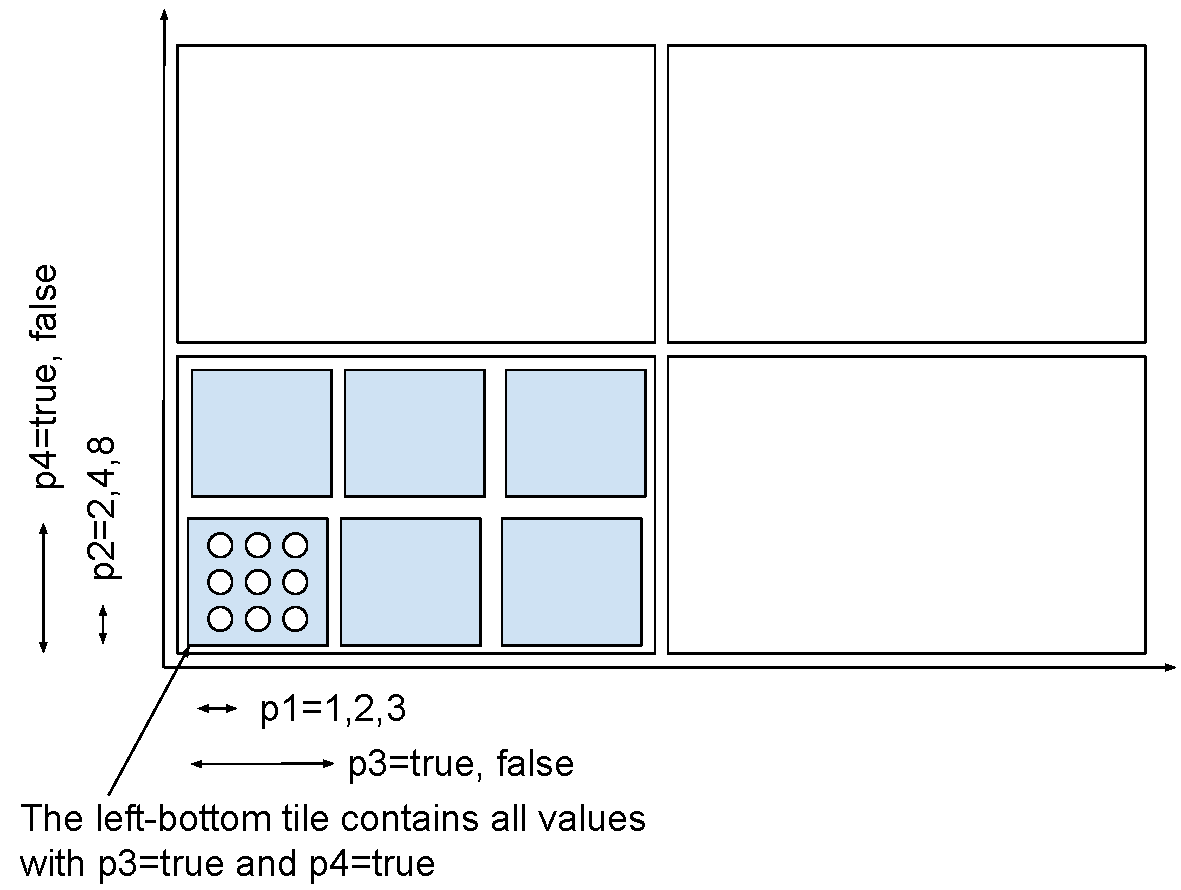
\includegraphics[width=0.45\textwidth]{tiledgraph}
    \caption{Tiled Heat Map.}
    \vspace{-.1in}
    \label{fig:tiledgraph}
\end{figure}

To achieve this goal, we design and develop a tool to visualize high-dimensional
data on a figure called Tiled Heat Map (Figure~\ref{fig:tiledgraph}):
assuming the system has $n$ parameters from $p_1$
to $p_n$, in the first iteration, our tool picks two parameters (e.g., $p_1$ and $p_2$) and groups all
data with the same $p_3$ to $p_n$; then it is able to draw each group
on a 2D figure called a ``tile'' since each group only contains two parameters $p_1$ and $p_2$.
In the second iteration, our tool picks two additional parameters (e.g., $p_3$ and $p_4$)
and groups tiles with the same $p_5$ to $p_n$ into a super-tile. It repeats
this procedure until it covers all parameters (the last iteration may just pick one parameter). 
Our tool uses Matplotlib~\cite{matplotlib} as its plotting interface. 
Section~\ref{sec:cases} shows some real
Tiled Heat Maps we build.

\vspace{-.1in}
\paragraph{Order of parameters.}
Our tool needs to choose parameters in each iteration.
Among all the possible choices, we try to choose the one that causes
the final figure to be ``smooth'' for easy reading (i.e., large values are close
to each other and small values are close to each other). Formally, we define the following metric
to measure how ``smooth'' a figure is, assuming there are $n$ points in the figure,
and each point has a coordinate $(x_i, y_i)$ and a value $v_i$.

\begin{definition}

    $smoothness = |SpearmanCorrelation(D, V)|$
    
, in which

$D=\{\forall (i,j), d_{ij} = |x_i-x_j|+|y_i-y_j| \}$

$V=\{\forall (i,j), v_{ij} = |v_i-v_j|\}$


\end{definition}

% \todo{Miao, add a short description about Pearson Correlation}
% Pearson's correlation coefficient~\cite{pearsonCorr} is used to measure the linear correlation between two sets of data.
We use Spearman's correlation coefficient~\cite{spearmanCorr}, which is the Pearson's correlation~\cite{pearsonCorr} between two rank variables, to measure how well the relationship between $D$ and $V$ can be described using a monotonic function. We choose Spearman's correlation over Pearson's because the latter measures linearity, while we only care about monotonicity here.

Intuitively, a high smoothness value means the value difference between two points
is highly correlated with the distance between them. In other words,
points with very different values
are far away from each other and points with close values are close to each other,
which is exactly what we want.

Our tool tries all the possible orders of parameters to compute the smoothness of each order
and chooses the one with the highest smoothness. If the figure contains many points,
our tool samples a subset of them to compute the smoothness value. Assuming the target system has $p$ parameters, there
is a total of $p!$ choices: with a small $p$, iterating all choices is feasible: with a 
bigger $p$, we probably need to go for heuristic solutions. In our experiments, we
find iterating all is feasible.

\vspace{-.1in}
\paragraph{Choosing the value and color of each point.} 
The Tiled Heat Map can be used to present different types of values, such as the
raw throughput, the improvement of one system over another, etc.

In the Tiled Heat Map, we use a color
to represent the value of each point. 
By default, our tool first finds the minimal and maximal values, and
then evenly distributes all values among gray color \#CECECE to \#0A0A0A (we observe
colors very close to full black or white are hard to distinguish, so we try to avoid them).
However, just like most graph plotting tools, our tool allows
the user to specify a color for a value range manually.
In this paper, we use gray colors to meet
the requirement of the conference, and using more colors can often create
a more readable version.

\vspace{-.1in}
\paragraph{Limitations.}
As shown in the next section, we find the Tiled Heat Map is good at presenting the overall
trend about how parameter values (or a combination of parameter values) can affect
system performance. However, it is not very good at presenting the absolute value of
each data point or comparing values with a small difference (e.g., 10\%). Therefore,
we propose the Tiled Heat Map as a complement to traditional line or bar graphs.
Furthermore, although the Tiled Heat Map can typically show more information on
the same area, its capability is still limited by the number of pixels we can have:
when viewing it on a computer, this problem can be addressed by zooming in/out, which we find helpful, but
when printing it on paper, there is eventually going to be a limit.
Finally, we have tried the Tiled Heat Map on data with at most five dimensions
and it is likely that more dimensions will make the figure harder to read.

%\vspace{-.1in}
%\paragraph{Suggestions.}
%While our community has always required figures in a publication to be readable
%when printed on a black-white printer and without a magnifier, which is
%very understandable, we argue it is eventually limiting the capability
%of presenting the results from extensive evaluation. We suggest our community
%to consider the possibility of allowing large colored figures, maybe as
%supplemental materials, for readers who are interested.




\section{Case Studies}
\label{sec:cases}

This section discusses our experience in evaluating prior prototypes under
a wider range of settings, including both correctness and performance issues.
We try our best to fix these issues, but due to time constraints and the nature of debugging, we
are only able to fix a subset of them. Significant design-level changes are also out of the scope
of this paper.

\subsection{Correctness Issues}

\paragraph{Configuration issues.}

Many systems have hard-coded configuration parameters, which prevent extensive evaluation.

\begin{itemize}[leftmargin=*]

    \vspace{-.05in}
    \item Fixed memory allocation. Silo, Cicada, DrTM, and GAM allocate a fixed
    amount of memory. As a result, they fail if the experiments load more data,
    even if there is enough physical memory. Fixing these issues is often not
    as simple as changing a value, since some systems need to allocate memory 
    separately for different types of data 
    (e.g., Silo allocates a memory region for its underlying B\textsuperscript{+} tree nodes and database records, 
    plus a buffer region for each thread), and we had to manually tune the size of each part to
    maximize the total amount of data they can support.
    
    \vspace{-.05in}
    \item Fixed thread/warehouse ratio. DrTM assumes the
    number of threads is equal to the number of warehouses. When we test with
    more warehouses, this leads to significant performance degradation.
    We fixed this issue by modifying DrTM source
    code to allow a thread to access more than one warehouse. Janus
    has the same constraint but due to time constraints, we have not fixed it.
    
    \vspace{-.05in}
    \item Too many open files. In Janus, we met a problem that the server processes
    fail to start when we start many servers. After debugging, we find the root cause
    is that, in Janus, every server thread needs to open a socket to every other server
    thread, so when starting many servers, the number of sockets on one server becomes larger
    than the default maximal number of open files allowed by Linux. While fixing this issue is simple (i.e.,
    enlarge the maximal number of open files), such all-to-all socket creation may create
    scalability problems in a large deployment.
    
    \vspace{-.05in}
    \item Inappropriate timeout values. Many systems use timeout for different purposes, like
    detecting whether a node has failed or whether an experiment has failed. Under a new
    setting, however, the default timeout value sometimes becomes inappropriate, causing phenomena
    like a running experiment or a healthy node getting killed. We manually tune
    the timeout value when the default one does not work.
    
    \vspace{-.05in}
    \item Limit on message size. HERD relies on the RDMA inlining feature to improve
    performance, and this feature usually only allows messages smaller than 512B.
    This problem is admitted in the HERD paper, and a complete solution would be to design
    additional communication paths for larger messages. Since the additional path does not affect
    messages using the inlining feature, we have not implemented it.
    
\end{itemize}

Besides, a number of systems do not implement all the parameters we have tried.
For example,
%Cicada does not allow to tune the rate of cross warehouse transactions on TPC-C; 
TAPIR
uses one thread per server, so we cannot tune the number of threads; many systems can only
support two types of transactions in TPC-C. Fixing these issues requires much more effort
and thus is out of the scope of this paper. Furthermore, some issues are caused by the inherent limitation of these
works (e.g., in TPC-C, \emph{New-Order} and \emph{Payment} do not need range queries
but the other three types need).

We make the following observations and suggestions: 1) it is often not hard to find
a workaround after we know the root cause,
%(e.g., fixed memory allocation, limit on message size),
but it sometimes takes longer to diagnose the root cause since the error messages often do not directly point to the root cause.
Performing an extensive evaluation would help the researcher to identify and fix these issues,
and help later works to compare to this work. 2) A fundamental solution to these problems, however,
probably requires more thoughts (e.g., adaptive memory allocation, adaptive timeout, etc) and 
could be a research problem.
%3) If our community plans to encourage extensive evaluation, then we should have a consensus
%about which parameters should be tuned, at least for those very popular benchmarks, so that different
%works can be compared under the same settings.

\begin{figure*}[ht]
    \centering
     \begin{subfigure}[t]{0.45\textwidth}
         \centering
         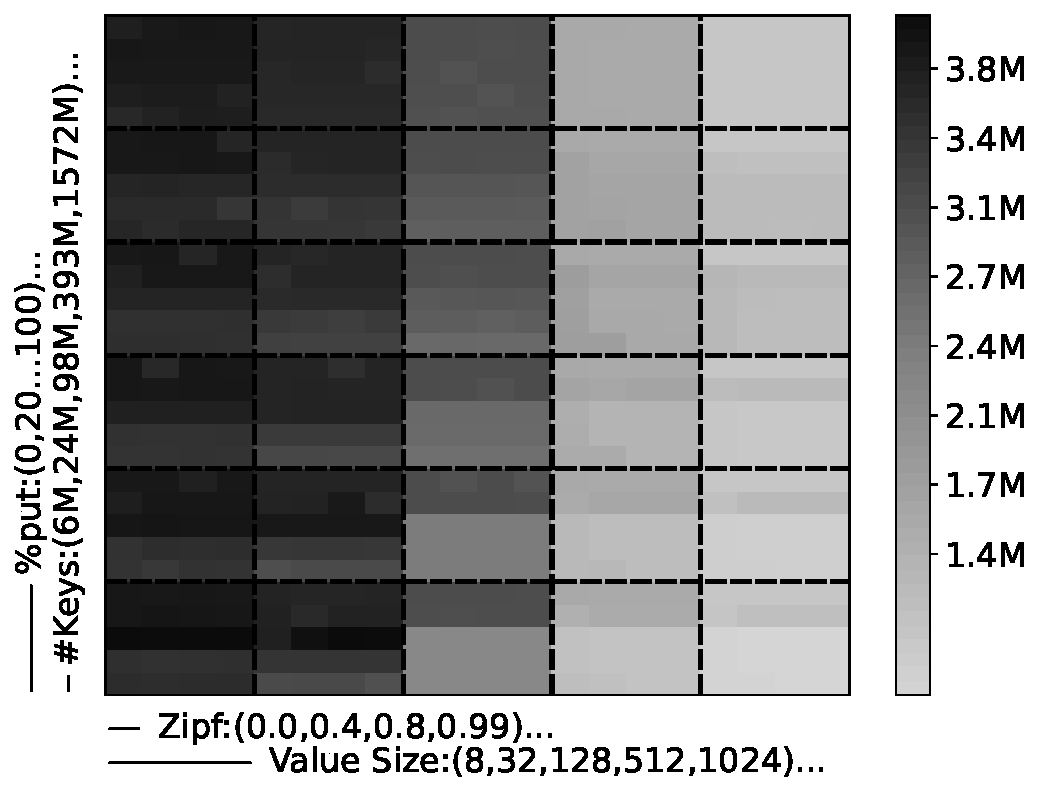
\includegraphics[width=\textwidth]{fig/herd/herd_ycsb.pdf}
         \caption{Per core throughput of HERD YCSB.}
         \label{fig:herd-throughput}
     \end{subfigure}
~
     \begin{subfigure}[t]{0.45\textwidth}
         \centering
         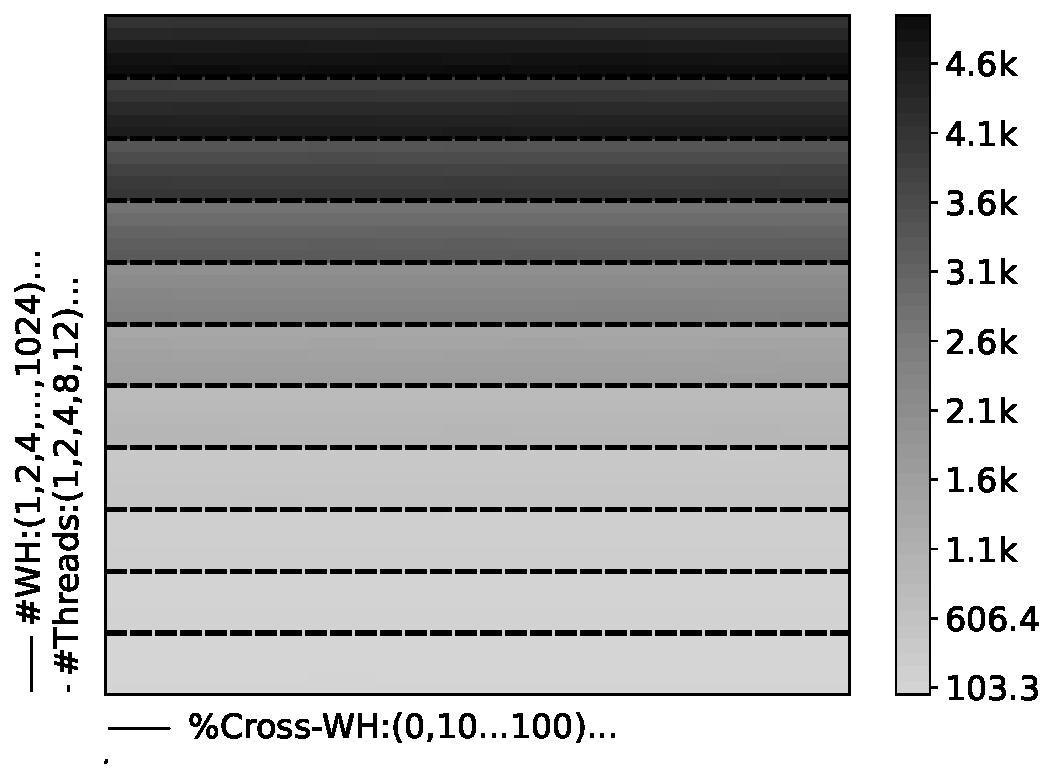
\includegraphics[width=\textwidth]{fig/aria/Aria_tpcc.pdf}
         \caption{Per core throughput of Aria TPC-C.}
         \label{fig:aria-throughput}
     \end{subfigure}
     
    \begin{subfigure}[t]{0.45\textwidth}
         \centering
         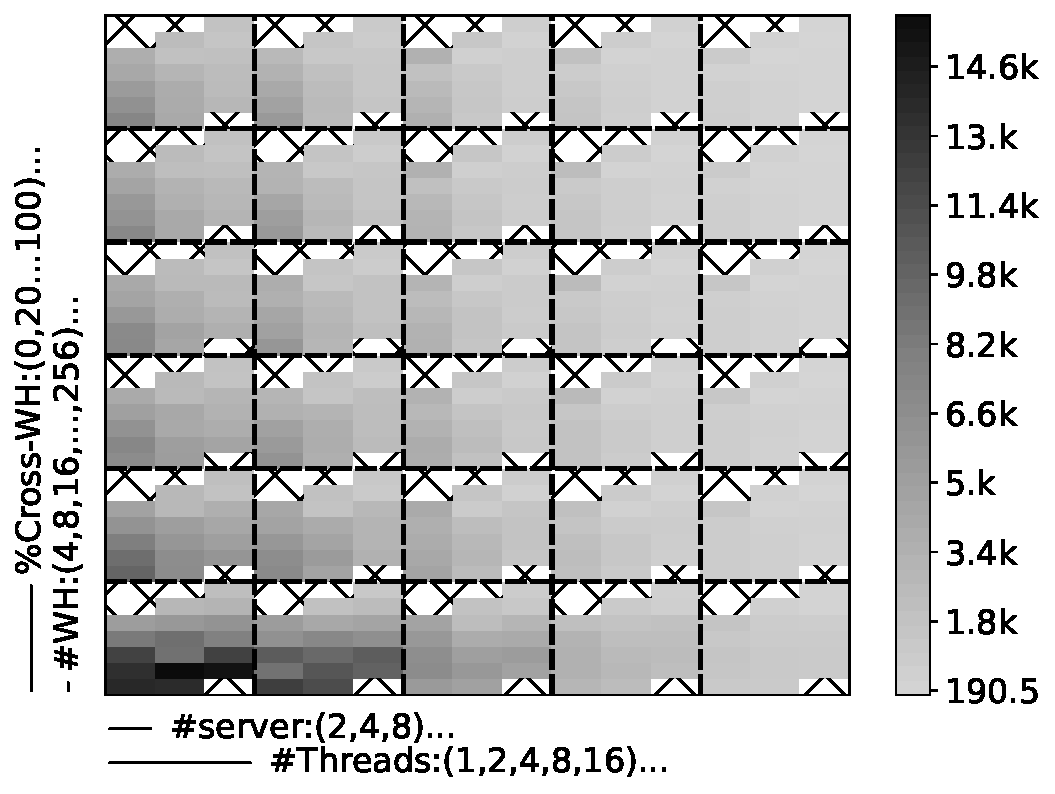
\includegraphics[width=\textwidth]{fig/gam/gam_tpcc.pdf}
         \caption{Per core throughput of GAM TPC-C.}
         \label{fig:gam-throughput}
     \end{subfigure}
     ~
     \begin{subfigure}[t]{0.45\textwidth}
         \centering
         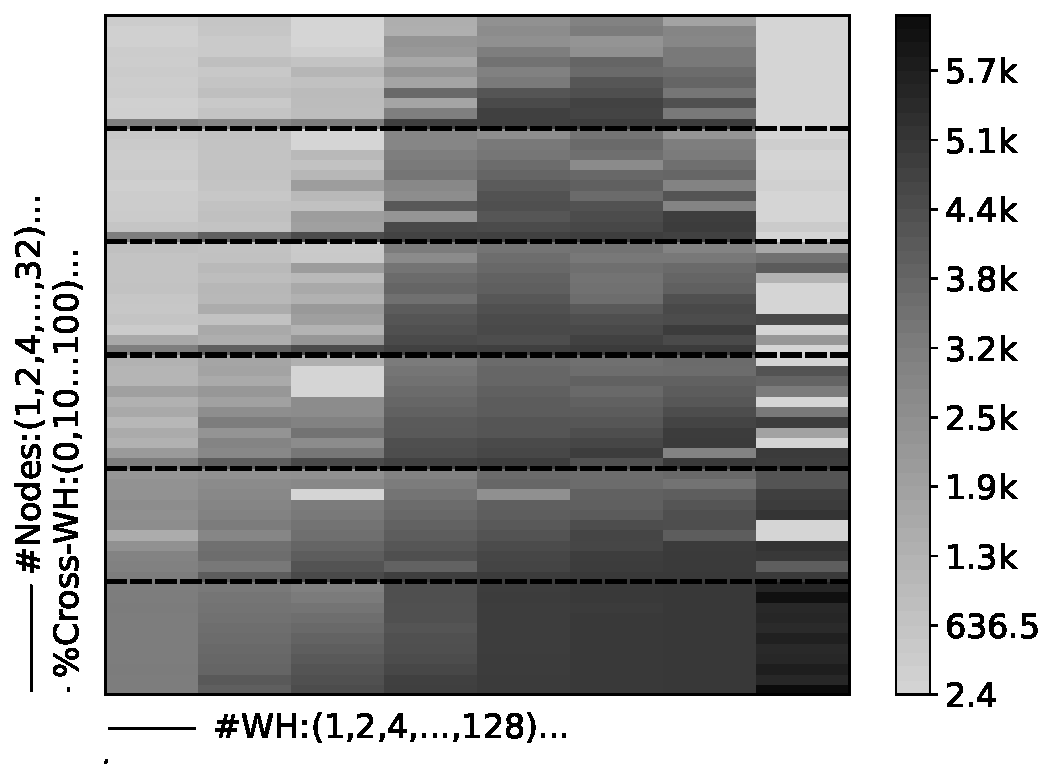
\includegraphics[width=\textwidth]{fig/calvin/Calvin_tpcc.pdf}
         \caption{Per core throughput of Calvin TPC-C.}
         \label{fig:calvin-throughput}
     \end{subfigure}
     %~
     %begin{subfigure}[t]{0.45\textwidth}
     %    \centering
     %    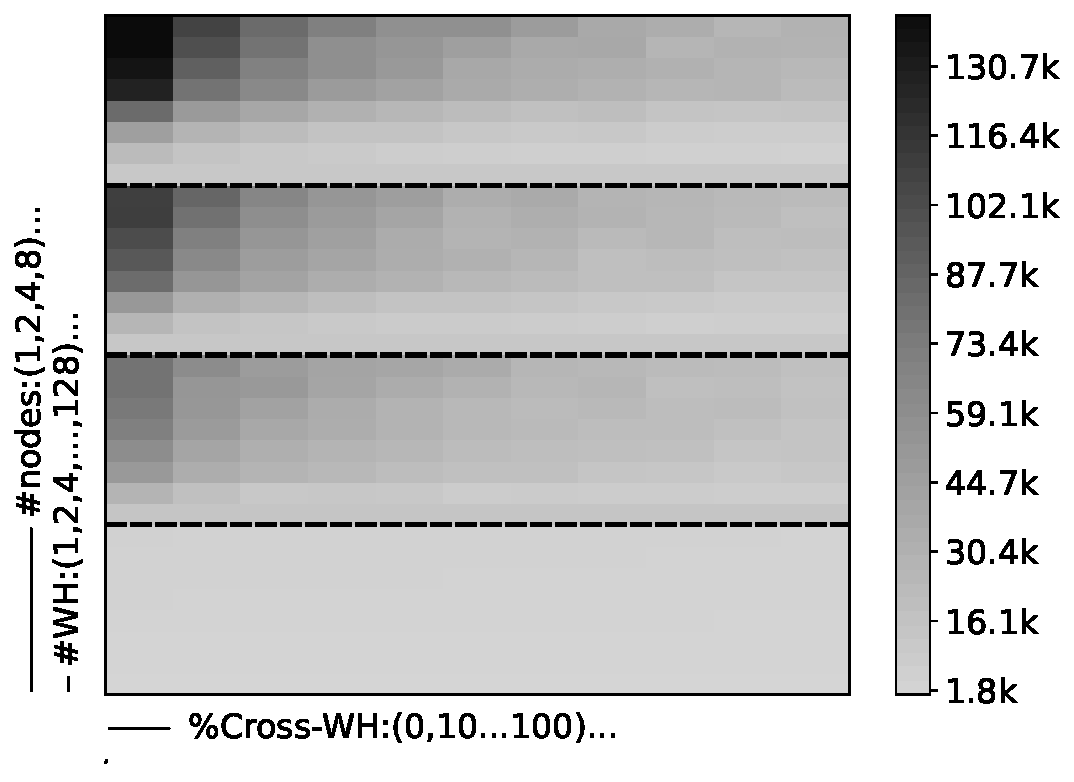
\includegraphics[width=\textwidth]{fig/aria/Calvin2-distributed-tpcc.pdf}
     %    \caption{Per core throughput of Calvin-2 from Aria TPC-C.}
     %    \label{fig:calvin2-throughput}
     %\end{subfigure}
     
     \caption{Systems with stable and unstable performance (white X indicates settings we canot run).}
     \vspace{-.1in}
     \label{fig:stable}
\end{figure*}

\vspace{-.1in}
\paragraph{Buggy or Incomplete Implementation.}

A few other issues are caused by bugs or incomplete implementation.
Due to the well-known difficulty of debugging non-deterministic issues,
we have not been able to diagnose the root cause of all of them, and
we report what we find.

\begin{itemize} [leftmargin=*]

    \vspace{-.05in}
    \item Segmentation fault. In Calvin, we find a number of settings cause
    abnormally low throughput, which further causes the bad prediction accuracy as
    shown in Section~\ref{sec:regression}. Our investigation shows these settings cause
    a segmentation fault in the middle, but the experiments still calculate the throughput
    by dividing the number of finished transactions by the total experiment time, which
    results in very low throughput. We further investigate the reason for the segmentation
    fault and find it is caused by the inappropriate handling of NULL value returned
    by set lookup, which is more likely to happen under certain settings. We are able
    to fix this issue to avoid segmentation fault but we find our fix leads to other problems.
    Since we cannot find an easy fix and Aria has already implemented a more predictable version of Calvin,
    we finally give up fixing the original version of Calvin.

    \vspace{-.05in}
   \item Lock implementation. Silo implements a competitor called PartitionedStore as
    a comparison. When testing PartitionedStore with more settings, we find the experiments
    cannot finish under certain settings. Our investigation finally traces the problem to the
    customized lock implementation of PartitionedStore: sometimes a thread cannot acquire a lock even if the
    previous owner has released the lock. We are not able to fully locate the root cause but
    we find this problem is highly likely to be correlated with the data alignment in PartitionedStore:
    this problem only happens under settings whose total size of locks is a multiple of page size,
    and by artificially adding a few bytes, we can see the problem does not happen anymore.

	\vspace{-.05in}
    \item Incomplete recovery. In TAPIR experiments we find sometimes the experiments cannot finish.
    By looking at their logs, we find these experiments trigger a timeout in the middle, probably
    due to short timeout intervals, and then trigger failure recovery. But since TAPIR does not implement
    the recovery protocol, the whole system cannot make progress. As discussed above, we enlarge the
    timeout value to avoid triggering failure recovery.
    
\end{itemize}

This type of issue is perhaps unavoidable since it is unrealistic to expect a research
prototype to be as stable and complete as a mature software and even a mature software can hardly be bug-free.
We believe the bottom line is that, by extensive evaluation, we can be aware of these issues
and have sufficient mechanisms to detect their manifestation.
Of course, if a bug frequently happens, it is better to be fixed.




\begin{figure*}[ht]
    \centering
     \begin{subfigure}[t]{0.45\textwidth}
         \centering
         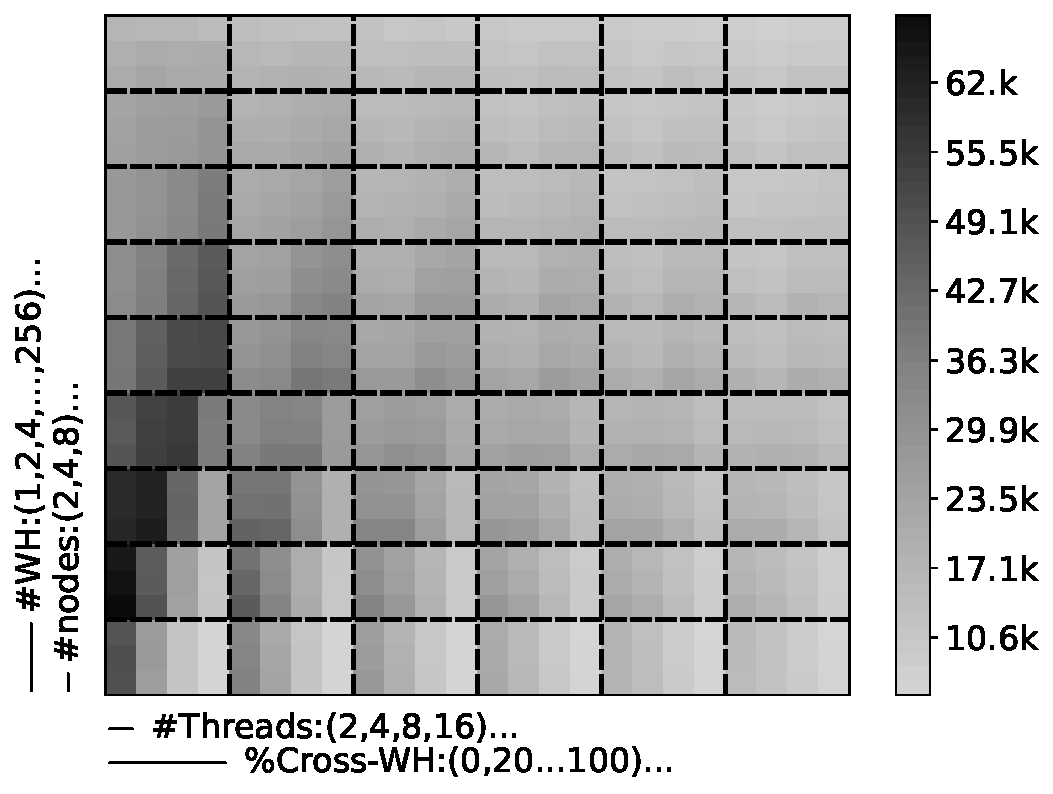
\includegraphics[width=\textwidth]{fig/drtm/drtm_tpcc.pdf}
         \caption{DrTM TPC-C throughput per server core.}
         \label{fig:drtm-throughput}
     \end{subfigure}
    ~
     \begin{subfigure}[t]{0.45\textwidth}
         \centering
         
\includegraphics[width=\textwidth]{fig/silo/silo_ycsb.pdf}
         \caption{Silo YCSB throughput per server core.}
         \label{fig:silo-ycsb-throughput}
     \end{subfigure}
     
     
     \begin{subfigure}[t]{0.45\textwidth}
         \centering
         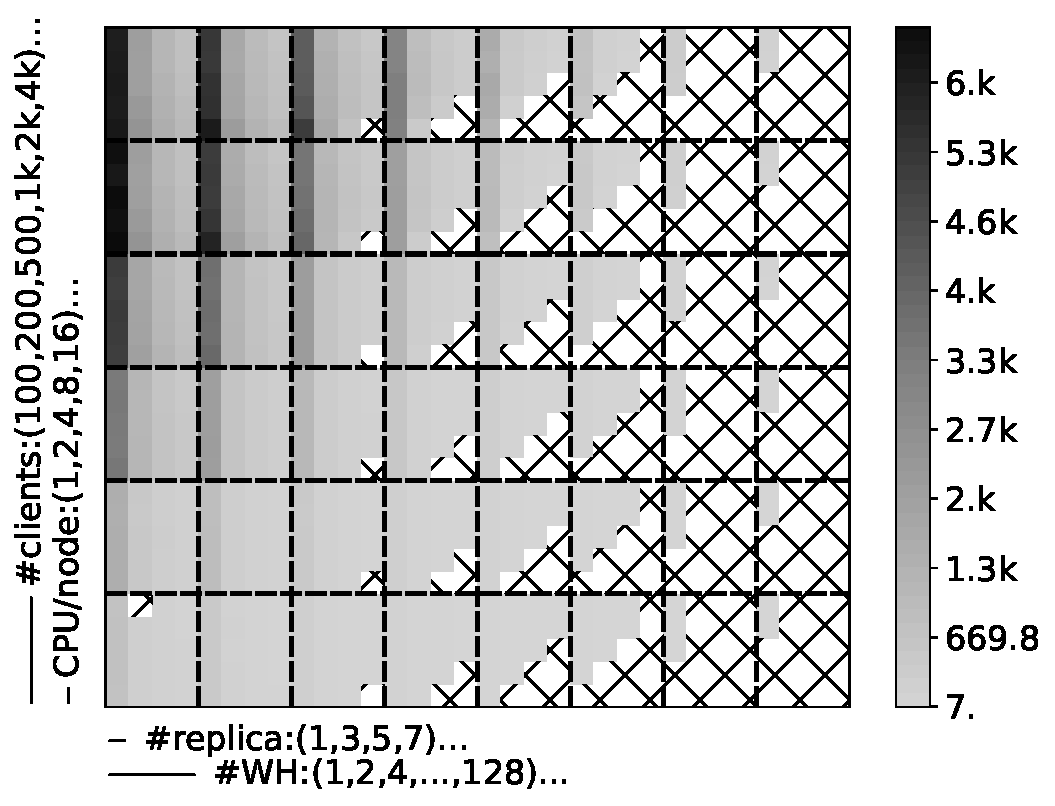
\includegraphics[width=\textwidth]{fig/janus/Janus_tpcc.pdf}
         \caption{Janus TPC-C throughput per server core.}
         \label{fig:janus-throughput}
     \end{subfigure}
     ~
     \begin{subfigure}[t]{0.45\textwidth}
         \centering
         
\includegraphics[width=\textwidth]{fig/janus/2PL_tpcc.pdf}
        \caption{2PL TPC-C throughput per server code.}
        \label{fig:2pl-throughput}
     \end{subfigure}
     
     \caption{Comprehensive analysis of system performance. White Xs indicate settings we cannot run due to resource constraints.}
     \vspace{-.1in}
     \label{fig:comprehensive}
\end{figure*}


\subsection{Comprehensive Performance Analysis and Comparison}


In this section, we present how
extensive evaluation helps to reveal performance issues
and allows a more comprehensive performance comparison.
Due to space limitation, we discuss a subset of results
here and publish all figures at our anonymous website~\cite{FigureSite}.

\vspace{-.1in}
\paragraph{Predictable vs unpredictable performance.}



As shown in Section~\ref{sec:regression}, some systems have highly predictable
performance and some are less predictable. The Tiled Heat Map can provide
a direct illustration of such problems.

As shown in Figure~\ref{fig:stable}, HERD has a very regular performance pattern:
throughput decreases with larger KVs, which is as expected; more KVs
improve the throughput by a small extent; other parameters do not seem
to have a strong impact on throughput. Aria and GAM are two other examples with
a very regular performance pattern: that's why we find it surprising
that the prediction accuracy on Aria is not good (Section~\ref{sec:regression}).

Calvin, on the other hand, has a
less regular pattern as one can see there are often abrupt throughput
changes between adjacent settings. By looking at its Tiled Heat Map, we investigate
these abnormal points, which lead to our discovery in the previous section. 
The Calvin implementation from the Aria work has a much more regular pattern.
%as shown in Figure~\ref{fig:calvin2-throughput}.




\vspace{-.1in}
\paragraph{A Comprehensive Understanding of System Performance.}



Extensive evaluation with the Tiled Heat Graph
has helped to reveal performance characteristics in a more comprehensive manner and
some of them are potential design issues.

Figure~\ref{fig:drtm-throughput} shows the throughput of DrTM, which reveals
several patterns: in general, more distributed transactions lead to lower
throughput per core, which is expected; the number of nodes does not have a
strong impact on throughput per core, which shows DrTM has good scalability
by adding more nodes; the number of warehouses and the number of threads combined
create the step-like pattern, because more threads than warehouses will create
a high contention, which results in lower throughput. However, apart from all these
explainable patterns, we find one pattern hard to explain: further increasing the
number of warehouses beyond the number of threads causes a quite significant drop
of throughput per core.
We use \emph{perf}~\cite{perf} to profile DrTM and find, with more warehouses,
DrTM spends more time on indexing. This is because DrTM uses tree indexes, and
with more data, the trees grow taller and require more time for updating and searching.

Silo has exactly the same issue as shown in Figure~\ref{fig:silo-ycsb-throughput}:
it uses Masstree as the index and since the tree grows taller with more KVs, tree update
takes longer, which causes performance degradation with more KVs.

A classic solution to this problem is to shard the data and use an index for each
shard~\cite{Decandia07Dynamo,chang06bigtable,Lee2021ShardManager}. Actually among the systems we tested,
HERD, Star, and even Silo's competitor PartitionedStore perform data partition as well.
These examples show the risk without extensive evaluation:
if a later work needs to compare with DrTM or Silo under a setting with more KVs,
its author has to optimize the prior work for a fair comparison; even worse,
if its author is unaware of these issues, s/he may make an unfair comparison.
Later we will show how this issue affects the comparison between Silo and
its competitor PartitionedStore.


%We make two comments: 1) sharding in some cases is not as straightforward as
%just partitioning data, since the system may need to handle range queries,
%load balancing across shards, etc. For such systems, the overhead of
%indexing may change the bottleneck of the system. 2) obviously it is not
%fair to compare systems using and not using sharding.

%As shown in Figure~\ref{fig:gam-throughput}, GAM has a similar pattern that
%it reaches the highest throughput with 8-16 warehouses and the throughput decreases
%with more warehouses. The reason is that GAM heavily relies on caching for
%best performance: when there are many warehouses,
%cache becomes less effective since TPC-C is dominated by random accesses.
%We don't know a good solution for this problem, but on the other hand, it may not be
%a good idea to evaluate a cache system with a random workload in the first place.

Figure~\ref{fig:janus-throughput} and Figure~\ref{fig:2pl-throughput} show the throughput of Janus
and its competitor two-phase locking (2PL). They have the configuration
constraint that $\#CPUsPerNode \times \#Nodes = \#replica \times \#WH$.
In other words, increasing \#WH will increase the number of nodes in these figures.
As shown in Figure~\ref{fig:janus-throughput}, Janus' per-core throughput grows
with more clients since too few clients will not be able to saturate the server;
its per-core throughput drops with more replicas, which is expected since more
replicas will incur more messages; its per-core throughput keeps stable when
adding more CPUs per node, which means it scales up quite well; however, when
adding nodes (i.e., warehouses), we can see its per-core throughput drops to some degree, which
means it does not scale out very well. We investigate these
experiments but do not find a clear bottleneck and we suspect the performance drop
is caused by Janus' construction of a global dependency graph, which may incur
more overhead when adding more nodes. How to improve the scalability
of a global dependency graph could be an interesting research topic.

Figure~\ref{fig:2pl-throughput} shows that 2PL has a very different pattern:
its per-core throughput drops with more replicas, which is expected and the same as
Janus; its combination of number of clients and number of warehouses shows the
step pattern, which indicates 2PL can achieve the highest throughput if its \#clients and \#WH
has a fixed rate. This is due to the fact that too few clients cannot saturate
the server and too many clients will cause many deadlocks. Finally, we observe 2PL
can both scale up and scale out pretty well, which is reasonable since 2PL has no
inherent bottleneck.

\vspace{-.1in}
\paragraph{A Comprehensive Comparison.}

\begin{figure}[t]
    \centering
    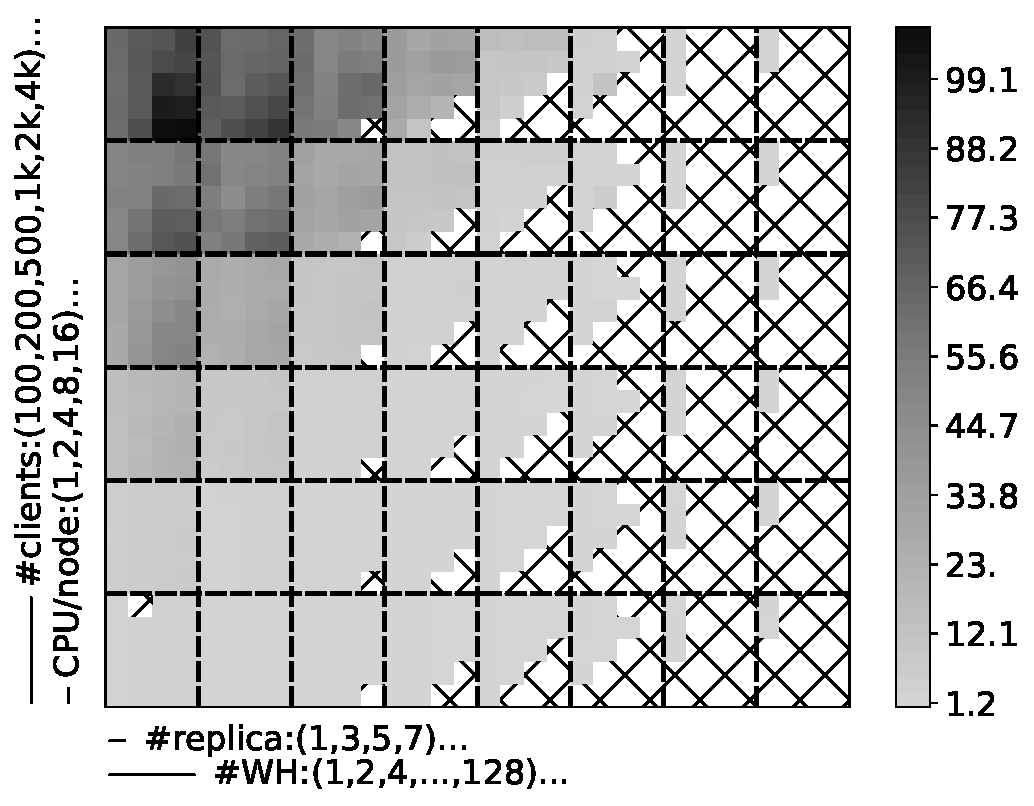
\includegraphics[width=0.45\textwidth]{fig/janus/[comp]Janus-vs-2PL_tpcc}
    \caption{Janus over 2PL. White Xs indicate settings we cannot run due to resource constraint.}
    \vspace{-.1in}
    \label{fig:janus_vs_2pl}
\end{figure}

%\begin{figure}[t]
%    \centering
%    
\includegraphics[width=0.45\textwidth]{fig/janus/2PL_tpcc.pdf}
%    \caption{Throughput of 2PL}
%    \label{fig:2pl}
%\end{figure}

\begin{figure}[t]
    \centering
    
\includegraphics[width=0.45\textwidth]{fig/silo/[comp]Silo-vs-PartitionedStore_tpcc}
    \caption{Silo over PartitionedStore}
    \vspace{-.1in}
    \label{fig:silo-vs-partitionedstore}
\end{figure}

Finally, we use two examples to show how extensive evaluation can allow
a more comprehensive evaluation. To compare two works A and B, we use the Tiled
Heat Map to draw throughput of A over throughput of B.

Figure~\ref{fig:janus_vs_2pl} shows the comparison between Janus and 2PL. As one can
see, Janus can achieve the highest improvement on the top left corner (i.e, more clients
and fewer warehouses), which incurs the highest contention level; its improvement
decreases with more warehouses, because as discussed above, Janus does not scale out
very well but 2PL does. It would be interesting to see the trend in a large setting
but unfortunately
we do not have enough machines for that.

%\begin{figure}[t]
%    \centering
%    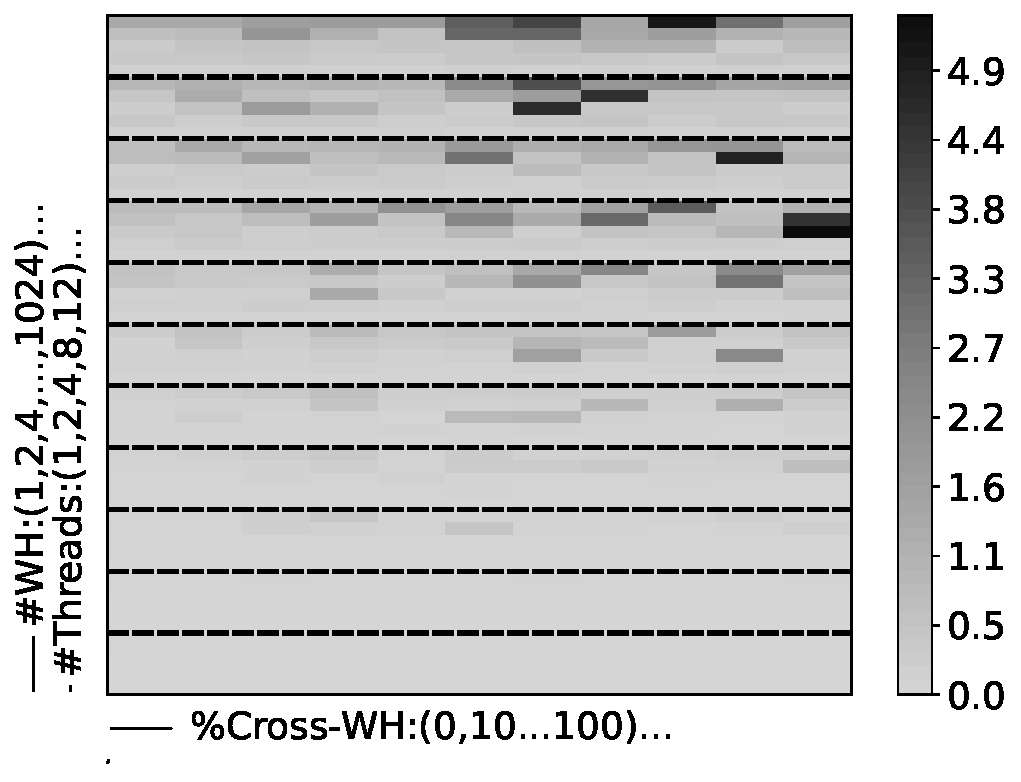
\includegraphics[width=0.45\textwidth]{fig/aria/[comp]aria-vs-Pwv_tpcc}
%    \caption{Aria over Pwv}
%    \label{fig:aria-vs-pwv}
%\end{figure}

%\begin{figure}[t]
%    \centering
%    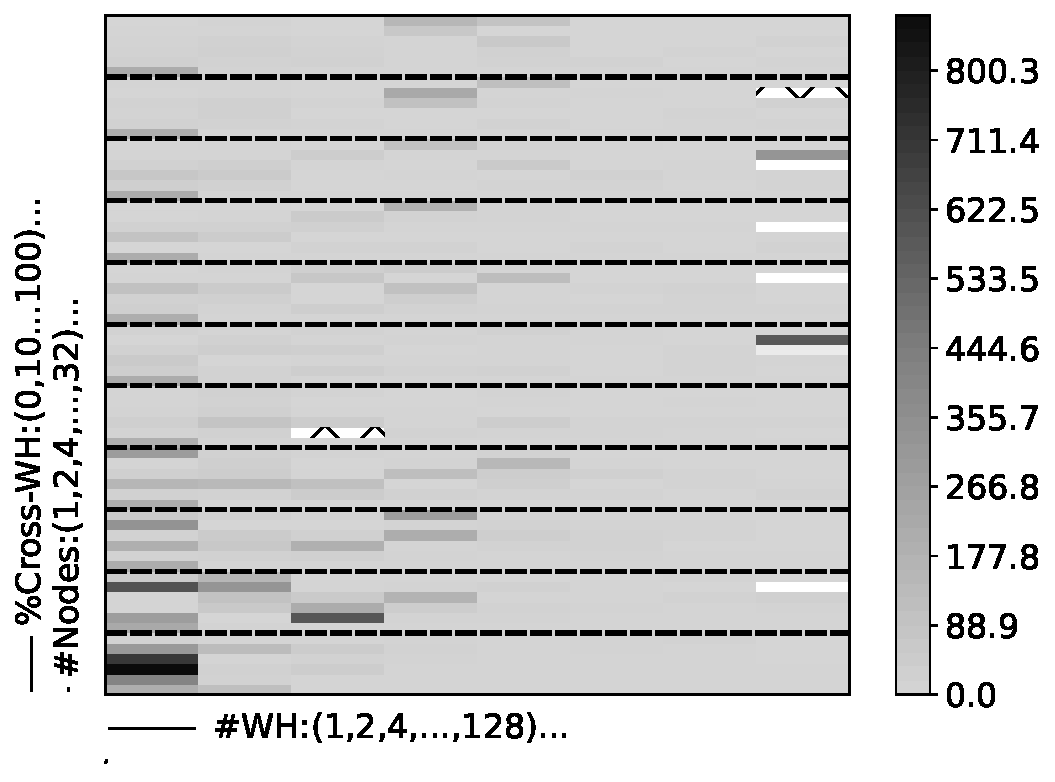
\includegraphics[width=0.45\textwidth]{fig/calvin/[comp]Calvin-vs-2pl_tpcc}
%    \caption{Calvin over 2PL}
%    \label{fig:calvin-vs-2pl}
%\end{figure}

%\begin{figure}[t]
%    \centering
%    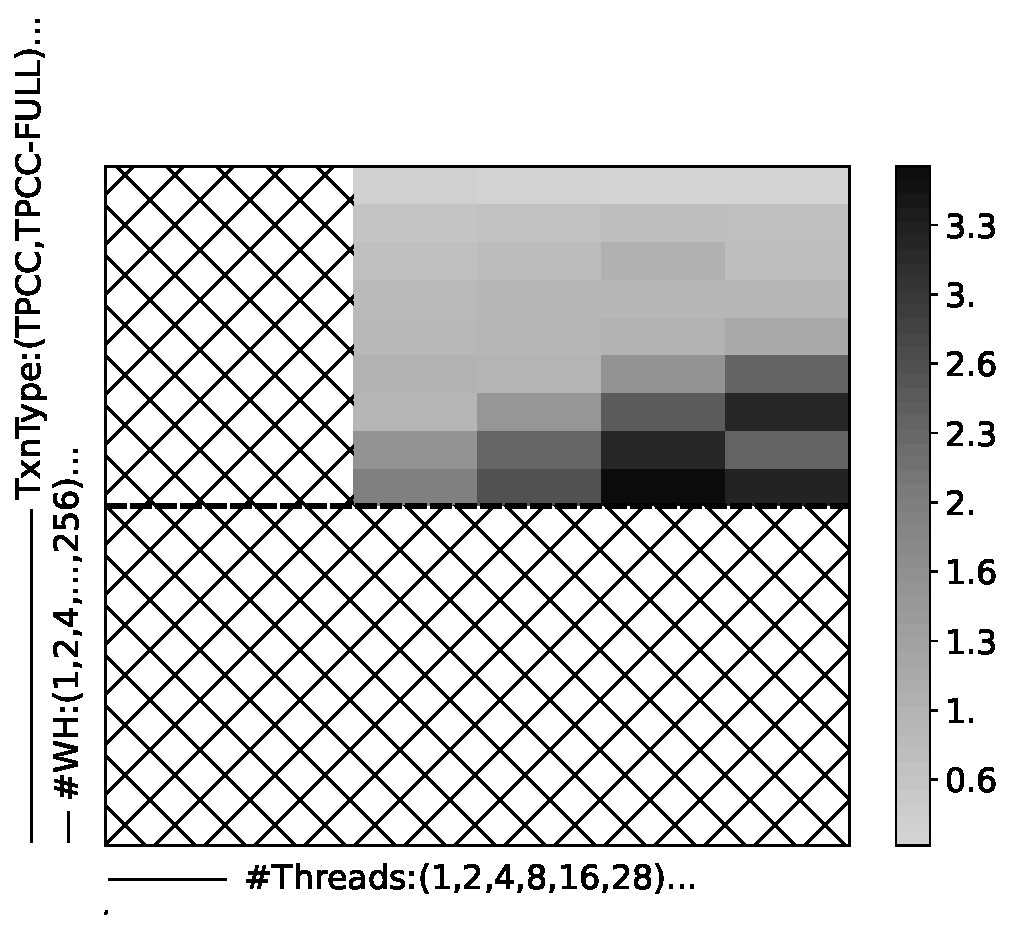
\includegraphics[width=0.45\textwidth]{fig/cicada/[comp]cicada-vs-MOCC_tpcc}
%    \caption{Cicada over MOCC}
%    \label{fig:cicada-vs-MOCC}
%\end{figure}




Figure~\ref{fig:silo-vs-partitionedstore} shows the comparison between
Silo and its competitor PartitionedStore. In general, we can see the improvement drops with more
warehouses, fewer threads, and fewer cross-warehouse transactions. Our analysis shows two reasons.
First, Silo targets addressing contentions and contention level decreases with more
warehouses, fewer threads, and fewer cross-warehouse transactions, so Silo's relative
benefit becomes smaller. Second, as mentioned above, Silo does not partition data so
its tree index grows taller with more data; PartitionedStore partitions data and thus
does not have this problem. Among these two reasons, the first reason is the one we are
interested in since Silo targets addressing contentions; the second one does not seem
to be a fundamental limitation of Silo and is diminishing the true improvement of Silo.

\vspace{-.1in}
\paragraph{Memory consumption.}
From the extensive evaluation, we observe the memory consumption of these
systems vary a lot. We measure the memory consumption
per warehouse under the TPC-C workload: for systems that perform customized
memory allocation, we set a maximal memory limit
and then increase the number of warehouses, till the system crashes; for systems
relying on malloc, we use the \emph{sysinfo} call to get memory consumption
before and after loading a warehouse. Our measurement shows that 
their per-warehouse memory consumption varies significantly: 33MB for Calvin, 59MB for Aria, 64MB for Star and DrTM,
330MB for Silo, 360MB for Cicada, and over 600MB for GAM.
Such gap
is caused by the difference among their exact data to populate, their
data layouts, and their index formats.

For in-memory systems, memory consumption is certainly an important factor and
we suggest to at least report the memory consumption numbers. Of course how
to reduce memory consumption can be a research topic as well.


\vspace{-.1in}
\paragraph{Effects of Extensive Evaluation.}
Most of the issues discussed in this section are not obvious in the original
settings of their corresponding papers: DrTM assumes the number of threads
is equal to the number of warehouses and tests with at most 28 warehouses,
Silo uses a fixed 160M key-value pairs in YCSB and uses at most 32 warehouses
in TPC-C. Therefore, for these two systems, the trend that
more data lead to performance degradation is unclear. Janus tests with 6 warehouses,
so the scalability issue is unclear as well.
Extensive evaluation and proper visualization can help to reveal these problems
and facilitate future comparison.




\section{Summary of Suggestions}

This section summarizes the suggestions:

\begin{itemize}[leftmargin=*]
    
    \vspace{-.05in}
    \item As shown in this work, extensive evaluation has the benefits of
    exposing both implementation and design issues. Since these benefits well align
    with the goals of artifact evaluation, maybe we should encourage extensive
    evaluation during artifact evaluation.
    
    \vspace{-.05in}
    \item Sampling and regression is a feasible solution to reduce the cost of
    extensive evaluation. We could gradually sample and test more settings until
    the prediction error becomes stable. If the error is still high, it may indicate
    performance anomalies, which require further investigation.
    
    \vspace{-.05in}
    \item To facilitate extensive evaluation, our community may have a discussion about
    tunable parameters and their values for popular benchmarks.
\end{itemize}

\section{Related Work}
  
%Many existing studies have been discussed throughout the paper. In this section,
%we mainly focus on discussing other related work in the following two categories.

\vspace{-.1in}
\paragraph{Benchmarks.}
Many areas have well-established benchmarks for performance evaluation and comparison,
such as the TPC series~\cite{tpcurl}, SmallBank~\cite{alomari2008cost}, YCSB~\cite{Cooper2010YCSB},
fio~\cite{fio-repo}, the SPEC series~\cite{specurl},
HPL~\cite{hplurl}, HPCG~\cite{hpcg}, Graph500~\cite{graph500url},
MLPerf~\cite{mlperf-train,mlperf-infer}, DAWNBench~\cite{DAWNBench} and many others.
Most of these benchmarks have restrictions about what parameters can be tuned and what values can be used
for these parameters.
While this work focuses on
TPC-C and YCSB, we plan to perform a similar study on other
benchmarks in the future.

%\noindentparagraph{Database and key-value stores.}

\vspace{-.1in}
\paragraph{Reproducibility.} 
To improve code quality and facilitate future research, our community has encouraged
research papers to verify their reproducibility through artifact evaluation~\cite{osdi-repro,sosp-repro,eurosys-repro,vldb-repro,sigmod-repro}.
In the meantime, many works study how to improve the reproducibility of research
prototypes. For example, CloudLab studies the performance variability of its experiments
and proposes guidelines to reduce such variability~\cite{Maricq2018Variability};
a recent work studies how cloud-based big data workload can be affected by network variability~\cite{alex-nsdi20};
Fursin discussed the challenges and solutions from his experience of reproducing 150+ research
papers~\cite{fursin-2021};
Ursprung~\cite{lukas-vldb20} studies how to improve the reproducibility of data science workloads.
%The key idea of Ursprung is to transparently capture provenance and build lineage to automatically track static and runtime configuration parameters of data science pipelines. With Ursprung, the authors hope to improve the reproducibility of data science workloads.
%
Compared to these efforts, our work further argues that, for the purpose of
improving code quality and facilitating future research, we should encourage
extensive evaluation to cover a wider range of settings.

\vspace{-.1in}
\paragraph{Regression/Machine learning for systems.} 
%Regression analysis aims to estimate the relation between one dependent variable and multiple independent variables. 
%Regression is usually used to predict %or forecast 
%the dependent values with the independent values by a linear or non-linear regression model. 
Regression or machine learning based methods have been gaining momentum in systems designs and optimizations.
%The most widely used regression model is linear regression, which represents a line that fits the data. In addition to linear regression model, non-linear regression is more complex, which substantially overlaps with the field of machine learning. 
For instance, many studies~\cite{yu-dac-asplos18,mr-advisor,rfhoc} propose to use regression-based algorithms to tune systems configurations to achieve better performance. 
Recent systems research successfully exploits machine learning methods for resource management~\cite{Quasar,JouleGuard,LLAMA,CALOREE}, scheduling~\cite{Paragon,Decima}, I/O optimizations~\cite{Vivace,linnos}, and so on.
Compared to these efforts, our work demonstrates that regression can be a feasible solution to reduce the cost of extensive evaluation.

%works under a variety of settings, some of which are beyond the ones used in the original papers. As discussed in Section~\ref{sec:questions},
%to support such extensive comparison, we suggest to introduce the idea of ``supporting extensive testing'' into artifact evaluation.
%\vspace{-.1in}
%\paragraph{Extensive evaluation.} A number of works did extensive experiments to understand the impact of different concurrency control
%features~\cite{Harding2017EvalDistributed,Wu2017EvalMem,Lim2017Cicada}.
%This work studies the feasibility of extensive evaluation in general, how to visualize evaluation results,
%and the benefits of performing extensive evaluation.

%Since they also use TPC-C and YCSB, their observations overlap with ours to some extent (e.g., contention level matters).
%However, because they have a different goal compared to this paper, there are a few key differences: first, for an apple-to-apple comparison,
%they re-implement different concurrency control features under the same framework; this paper, instead, tries to understand whether
%changing experiment settings will change the conclusion of the original work and thus has to re-produce original works. Second, they focus more on
%tuning concurrency control features but less on tuning benchmark parameters and our work has the opposite focus. Finally, our
%paper covers additional systems which explore different designs (e.g. Janus, HERD, etc).
%Among the works we studied,
%Cicada~\cite{Lim2017Cicada} did an extensive comparison, but only on in-memory database engines.
%However, the major difference from our work is we are focusing on how to perform fair comparisons among systems by properly using popular benchmarks in our community. Note that, this paper also shows that the reproducibility of our studied systems are reasonably good.

%found that our community regularly disregards the variability when running experiments in the cloud. Thus, it
\vspace{-.1in}
\paragraph{Visualizing high-dimensional data.}
Visualizing high-dimensional data is a classic research topic with a large volume of work.
However, most of them focus on how to find the structure within high-dimensional data
and map it onto a 2D figure. This paper has a completely different goal and thus cannot
re-use these works directly. We have tried two popular algorithms in this area t-SNE~\cite{tSNE} and UMAP~\cite{UMAP} on our data 
and do not find a meaningful output. 
%t-SNE and UMAP both map high-dimensional data into a low dimension space, but with different techniques. 
%tSNE uses the t-distributed variant of Stochastic Neighbor Embedding~\cite{SNE}, 
%while UMAP builds upon mathematical foundations related to the work of Belkin and Niyogi on
%Laplacian eigenmaps~\cite{UMAPbackground}.


\section{Conclusion}

This paper shows that sampling and regression is a feasible solution to reduce
the cost of extensive evaluation. Furthermore, it shows that extensive
evaluation can help to reveal configuration issues, bugs, and design
issues that do not manifest in the original settings and allow a comprehensive
performance analysis. Based on such results, we make recommendations
about how to improve artifact evaluation with extensive evaluation.
We plan to explore other benchmarks in different areas,
in particular those with more parameters, in the future.

\section*{Availability}
%-------------------------------------------------------------------------------

We have published all figures on our anonymous website~\cite{FigureSite}.
We will further publish our regression code, visualization tool, enhanced source
code of prior works, and raw evaluation data.





%-------------------------------------------------------------------------------
\bibliographystyle{plain}
\bibliography{LasrBibtex}

%%%%%%%%%%%%%%%%%%%%%%%%%%%%%%%%%%%%%%%%%%%%%%%%%%%%%%%%%%%%%%%%%%%%%%%%%%%%%%%%
\end{document}
%%%%%%%%%%%%%%%%%%%%%%%%%%%%%%%%%%%%%%%%%%%%%%%%%%%%%%%%%%%%%%%%%%%%%%%%%%%%%%%%

%%  LocalWords:  endnotes includegraphics fread ptr nobj noindent
%%  LocalWords:  pdflatex acks

